\documentclass[a4paper]{book}
\usepackage{makeidx}
\usepackage{graphicx}
\usepackage{multicol}
\usepackage{float}
\usepackage{listings}
\usepackage{color}
\usepackage{ifthen}
\usepackage[table]{xcolor}
\usepackage{textcomp}
\usepackage{alltt}
\usepackage{ifpdf}
\ifpdf
\usepackage[pdftex,
            pagebackref=true,
            colorlinks=true,
            linkcolor=blue,
            unicode
           ]{hyperref}
\else
\usepackage[ps2pdf,
            pagebackref=true,
            colorlinks=true,
            linkcolor=blue,
            unicode
           ]{hyperref}
\usepackage{pspicture}
\fi
\usepackage[utf8]{inputenc}
\usepackage{mathptmx}
\usepackage[scaled=.90]{helvet}
\usepackage{courier}
\usepackage{sectsty}
\usepackage[titles]{tocloft}
\usepackage{doxygen}
\lstset{language=C++,inputencoding=utf8,basicstyle=\footnotesize,breaklines=true,breakatwhitespace=true,tabsize=8,numbers=left }
\makeindex
\setcounter{tocdepth}{3}
\renewcommand{\footrulewidth}{0.4pt}
\renewcommand{\familydefault}{\sfdefault}
\begin{document}
\hypersetup{pageanchor=false}
\begin{titlepage}
\vspace*{7cm}
\begin{center}
{\Large rolisz framework \\[1ex]\large 0.0.1 }\\
\vspace*{1cm}
{\large Generated by Doxygen 1.7.4}\\
\vspace*{0.5cm}
{\small Wed Apr 6 2011 17:21:56}\\
\end{center}
\end{titlepage}
\clearemptydoublepage
\pagenumbering{roman}
\tableofcontents
\clearemptydoublepage
\pagenumbering{arabic}
\hypersetup{pageanchor=true}
\chapter{Todo List}
\label{todo}
\hypertarget{todo}{}
\label{todo__todo000001}
\hypertarget{todo__todo000001}{}
 
\begin{DoxyDescription}
\item[Namespace \hyperlink{namespacerolisz}{rolisz} ]Error handling function 

ORM 
\end{DoxyDescription}
\chapter{Namespace Index}
\section{Namespace List}
Here is a list of all namespaces with brief descriptions:\begin{DoxyCompactList}
\item\contentsline{section}{{\bf Roland} }{\pageref{namespace_roland}}{}
\item\contentsline{section}{{\bf rolisz} }{\pageref{namespacerolisz}}{}
\end{DoxyCompactList}

\chapter{Data Structure Index}
\section{Class Hierarchy}
This inheritance list is sorted roughly, but not completely, alphabetically:\begin{DoxyCompactList}
\item \contentsline{section}{base}{\pageref{classbase}}{}
\begin{DoxyCompactList}
\item \contentsline{section}{rolisz}{\pageref{classrolisz}}{}
\end{DoxyCompactList}
\item \contentsline{section}{databaseAdapter}{\pageref{interfacedatabase_adapter}}{}
\begin{DoxyCompactList}
\item \contentsline{section}{MySQLiDatabase}{\pageref{class_my_s_q_li_database}}{}
\end{DoxyCompactList}
\item \contentsline{section}{db}{\pageref{classdb}}{}
\item \contentsline{section}{router}{\pageref{classrouter}}{}
\item \contentsline{section}{table}{\pageref{classtable}}{}
\end{DoxyCompactList}

\chapter{Data Structure Index}
\section{Data Structures}
Here are the data structures with brief descriptions:\begin{DoxyCompactList}
\item\contentsline{section}{\hyperlink{classbase}{base} }{\pageref{classbase}}{}
\item\contentsline{section}{\hyperlink{classrolisz}{rolisz} }{\pageref{classrolisz}}{}
\end{DoxyCompactList}

\chapter{File Index}
\section{File List}
Here is a list of all files with brief descriptions:\begin{DoxyCompactList}
\item\contentsline{section}{C:/wamp/www/framework/{\bf base.php} }{\pageref{base_8php}}{}
\item\contentsline{section}{C:/wamp/www/framework/{\bf databaseAdapter.php} }{\pageref{database_adapter_8php}}{}
\item\contentsline{section}{C:/wamp/www/framework/{\bf misc\_\-functions.php} }{\pageref{misc__functions_8php}}{}
\item\contentsline{section}{C:/wamp/www/framework/{\bf plugin.php} }{\pageref{plugin_8php}}{}
\item\contentsline{section}{C:/wamp/www/framework/{\bf pluginStructure.php} }{\pageref{plugin_structure_8php}}{}
\item\contentsline{section}{C:/wamp/www/framework/{\bf rolisz.php} }{\pageref{rolisz_8php}}{}
\item\contentsline{section}{C:/wamp/www/framework/{\bf router.php} }{\pageref{router_8php}}{}
\item\contentsline{section}{C:/wamp/www/framework/{\bf table.php} }{\pageref{table_8php}}{}
\item\contentsline{section}{C:/wamp/www/framework/{\bf template.php} }{\pageref{template_8php}}{}
\item\contentsline{section}{C:/wamp/www/framework/plugins/{\bf acl.php} }{\pageref{acl_8php}}{}
\item\contentsline{section}{C:/wamp/www/framework/plugins/{\bf form.php} }{\pageref{form_8php}}{}
\end{DoxyCompactList}

\chapter{Namespace Documentation}
\hypertarget{namespacerolisz}{
\section{rolisz Namespace Reference}
\label{namespacerolisz}\index{rolisz@{rolisz}}
}


\subsection{Detailed Description}
\begin{DoxyAuthor}{Author}
Szabo Roland  Szabo Roland 2011 
\end{DoxyAuthor}
\begin{DoxyVersion}{Version}
0.0.0.3  public
\end{DoxyVersion}
\begin{DoxyAuthor}{Author}
Roland Szabo

Roland Szabo 
\end{DoxyAuthor}
\begin{Desc}
\item[\hyperlink{todo__todo000001}{Todo}]Error handling function 

ORM \end{Desc}

\chapter{Data Structure Documentation}
\section{base Class Reference}
\label{classbase}\index{base@{base}}
Inheritance diagram for base:\begin{figure}[H]
\begin{center}
\leavevmode
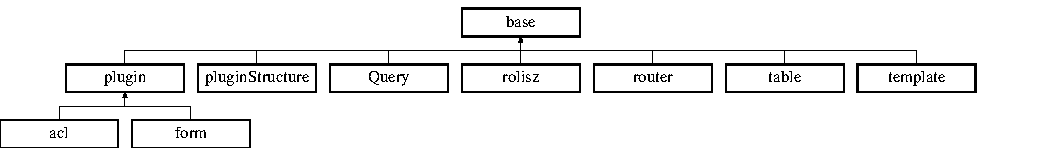
\includegraphics[height=1.981132cm]{classbase}
\end{center}
\end{figure}
\subsection*{Static Public Member Functions}
\begin{DoxyCompactItemize}
\item 
static {\bf get} (\$var)
\item 
static {\bf check} (\$var)
\item 
static {\bf set} (\$var, \$value=FALSE)
\end{DoxyCompactItemize}
\subsection*{Data Fields}
\begin{DoxyCompactItemize}
\item 
const {\bf AppName} = '{\bf rolisz} PHP framework'
\item 
const {\bf Version} = '0.0.3'
\item 
const {\bf Module} = 'Base class'
\item 
static {\bf \$plugins}
\item 
static {\bf \$executionPoints}
\end{DoxyCompactItemize}
\subsection*{Static Protected Attributes}
\begin{DoxyCompactItemize}
\item 
static {\bf \$global}
\end{DoxyCompactItemize}
\subsection*{Private Member Functions}
\begin{DoxyCompactItemize}
\item 
{\bf \_\-\_\-construct} ()
\end{DoxyCompactItemize}


\subsection{Detailed Description}
Base class for all the others in the framwork. Defines some framework details, global variables and setters and getters for framework variables. 

\subsection{Constructor \& Destructor Documentation}
\index{base@{base}!\_\-\_\-construct@{\_\-\_\-construct}}
\index{\_\-\_\-construct@{\_\-\_\-construct}!base@{base}}
\subsubsection[{\_\-\_\-construct}]{\setlength{\rightskip}{0pt plus 5cm}\_\-\_\-construct (
\begin{DoxyParamCaption}
{}
\end{DoxyParamCaption}
)\hspace{0.3cm}{\ttfamily  [private]}}\label{classbase_a095c5d389db211932136b53f25f39685}
Base constructor is private to disable creation of objects and to reinforce the usage of the singleton pattern. 

Reimplemented in {\bf plugin} \doxyref{}{p.}{classplugin_a095c5d389db211932136b53f25f39685}, {\bf pluginStructure} \doxyref{}{p.}{classplugin_structure_a095c5d389db211932136b53f25f39685}, and {\bf template} \doxyref{}{p.}{classtemplate_a095c5d389db211932136b53f25f39685}.



\subsection{Member Function Documentation}
\index{base@{base}!check@{check}}
\index{check@{check}!base@{base}}
\subsubsection[{check}]{\setlength{\rightskip}{0pt plus 5cm}static check (
\begin{DoxyParamCaption}
\item[{\$}]{var}
\end{DoxyParamCaption}
)\hspace{0.3cm}{\ttfamily  [static]}}\label{classbase_ae09ec448121b7c739ecd283675056e1f}
Checks if \$var variable has been set in the framework. 
\begin{DoxyParams}[1]{Parameters}
string & {\em \$var} & \\
\hline
\end{DoxyParams}

\begin{DoxyRetVals}{Return values}
{\em true} & \\
\hline
{\em false} & \\
\hline
\end{DoxyRetVals}
\index{base@{base}!get@{get}}
\index{get@{get}!base@{base}}
\subsubsection[{get}]{\setlength{\rightskip}{0pt plus 5cm}static get (
\begin{DoxyParamCaption}
\item[{\$}]{var}
\end{DoxyParamCaption}
)\hspace{0.3cm}{\ttfamily  [static]}}\label{classbase_a0e8f3e2708d9f0c6ee7b54599f57ea34}
Return the value of a framework variable or false if it was not found. 
\begin{DoxyParams}[1]{Parameters}
string & {\em \$var} & \\
\hline
\end{DoxyParams}

\begin{DoxyRetVals}{Return values}
{\em true} & \\
\hline
{\em false} & \\
\hline
\end{DoxyRetVals}
\index{base@{base}!set@{set}}
\index{set@{set}!base@{base}}
\subsubsection[{set}]{\setlength{\rightskip}{0pt plus 5cm}static set (
\begin{DoxyParamCaption}
\item[{\$}]{var, }
\item[{\$}]{value = {\ttfamily FALSE}}
\end{DoxyParamCaption}
)\hspace{0.3cm}{\ttfamily  [static]}}\label{classbase_adc76e59111cb34cf88726e6f3bd0be8b}
Set the value of a framework variable. If \$var param is a string, then a variable called \$var will have the value of \$value. If \$var is an array, it should be a key-\/pair value like this {\ttfamily  array('var\_\-name'=$>$'132','2ndvar'=$>$123) } 
\begin{DoxyParams}[1]{Parameters}
string | array & {\em \$var} & \\
\hline
mixed & {\em \$value} & \\
\hline
\end{DoxyParams}


\subsection{Field Documentation}
\index{base@{base}!\$executionPoints@{\$executionPoints}}
\index{\$executionPoints@{\$executionPoints}!base@{base}}
\subsubsection[{\$executionPoints}]{\setlength{\rightskip}{0pt plus 5cm}\$executionPoints}\label{classbase_a878a31351411a5b5d68c12c87c154084}
\index{base@{base}!\$global@{\$global}}
\index{\$global@{\$global}!base@{base}}
\subsubsection[{\$global}]{\setlength{\rightskip}{0pt plus 5cm}\$global\hspace{0.3cm}{\ttfamily  [static, protected]}}\label{classbase_aad844777d9d6beb4ca7c92d97afe7d27}
\index{base@{base}!\$plugins@{\$plugins}}
\index{\$plugins@{\$plugins}!base@{base}}
\subsubsection[{\$plugins}]{\setlength{\rightskip}{0pt plus 5cm}\$plugins}\label{classbase_a4ab51386acb82cd0a0066eac2567b2bd}
\index{base@{base}!AppName@{AppName}}
\index{AppName@{AppName}!base@{base}}
\subsubsection[{AppName}]{\setlength{\rightskip}{0pt plus 5cm}const {\bf AppName} = '{\bf rolisz} PHP framework'}\label{classbase_aab75444b144ffc4e972a9170e0a76ec0}
\index{base@{base}!Module@{Module}}
\index{Module@{Module}!base@{base}}
\subsubsection[{Module}]{\setlength{\rightskip}{0pt plus 5cm}const {\bf Module} = 'Base class'}\label{classbase_a2c348358c1db4bb5136855f7f31e1157}
\index{base@{base}!Version@{Version}}
\index{Version@{Version}!base@{base}}
\subsubsection[{Version}]{\setlength{\rightskip}{0pt plus 5cm}const {\bf Version} = '0.0.3'}\label{classbase_a62e44de9100d83ee01f5b4875b49a02b}


The documentation for this class was generated from the following file:\begin{DoxyCompactItemize}
\item 
C:/wamp/www/framework/{\bf base.php}\end{DoxyCompactItemize}

\hypertarget{interfacedatabase_adapter}{
\section{databaseAdapter Class Reference}
\label{interfacedatabase_adapter}\index{databaseAdapter@{databaseAdapter}}
}
Inheritance diagram for databaseAdapter:\begin{figure}[H]
\begin{center}
\leavevmode
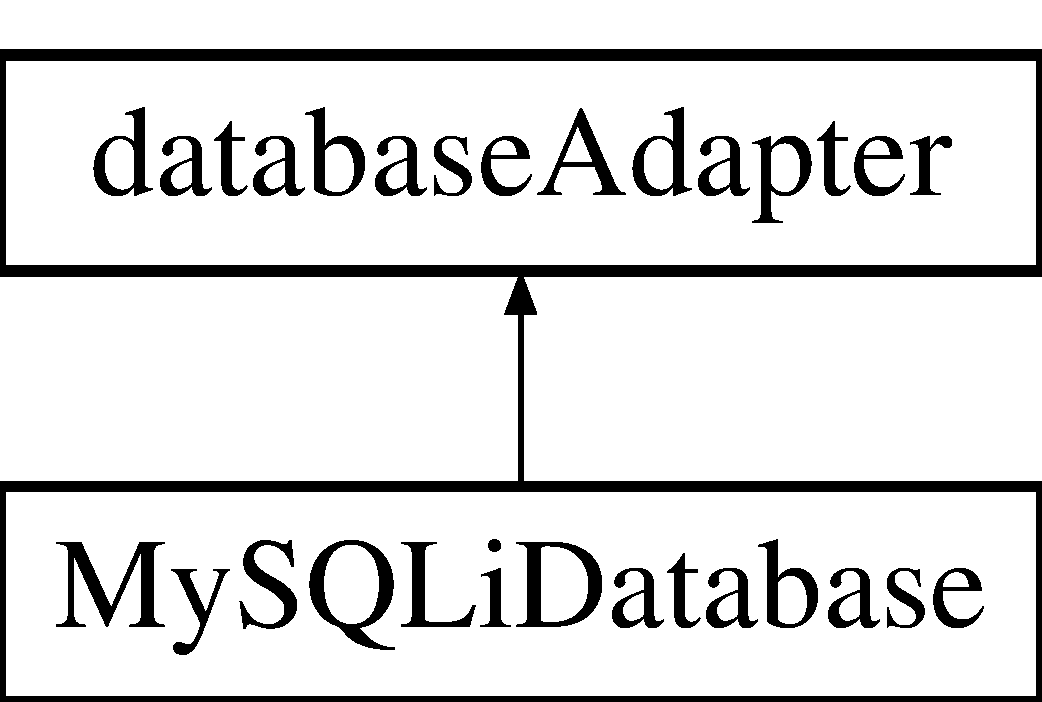
\includegraphics[height=2.000000cm]{interfacedatabase_adapter}
\end{center}
\end{figure}
\subsection*{Public Member Functions}
\begin{DoxyCompactItemize}
\item 
\hypertarget{interfacedatabase_adapter_a81fcddb424f13e0862ee3f7e1ea57ce9}{
{\bfseries \_\-\_\-construct} (\$host, \$username, \$password, \$db)}
\label{interfacedatabase_adapter_a81fcddb424f13e0862ee3f7e1ea57ce9}

\item 
\hypertarget{interfacedatabase_adapter_a4c4f3316747e665b9e02f6ddcba4117c}{
{\bfseries connect} (\$host, \$username, \$password)}
\label{interfacedatabase_adapter_a4c4f3316747e665b9e02f6ddcba4117c}

\item 
\hypertarget{interfacedatabase_adapter_a039ae2e8f2bf579fd75d9df8df87eee3}{
{\bfseries escapeValue} (\$value)}
\label{interfacedatabase_adapter_a039ae2e8f2bf579fd75d9df8df87eee3}

\item 
\hypertarget{interfacedatabase_adapter_a529385852efa66f19288496930ee5394}{
{\bfseries fetchRow} (\$query=false, \$type='assoc')}
\label{interfacedatabase_adapter_a529385852efa66f19288496930ee5394}

\item 
\hypertarget{interfacedatabase_adapter_a861f65695740a1d866ce1001f0ae706d}{
{\bfseries fetchAll} (\$query=false, \$type='assoc')}
\label{interfacedatabase_adapter_a861f65695740a1d866ce1001f0ae706d}

\item 
\hypertarget{interfacedatabase_adapter_a24ada5decce3d1b79cd82f5a90ccf404}{
{\bfseries getError} ()}
\label{interfacedatabase_adapter_a24ada5decce3d1b79cd82f5a90ccf404}

\item 
\hypertarget{interfacedatabase_adapter_ac73f1d8cddbdfc35ca442189378a073c}{
{\bfseries getInsertID} ()}
\label{interfacedatabase_adapter_ac73f1d8cddbdfc35ca442189378a073c}

\item 
\hypertarget{interfacedatabase_adapter_af37433a300db1f607ee789d22828a0a0}{
{\bfseries numRows} ()}
\label{interfacedatabase_adapter_af37433a300db1f607ee789d22828a0a0}

\item 
\hypertarget{interfacedatabase_adapter_acac8dfe61e7840f9a1e672ebede0be21}{
{\bfseries numAffected} ()}
\label{interfacedatabase_adapter_acac8dfe61e7840f9a1e672ebede0be21}

\item 
\hypertarget{interfacedatabase_adapter_ac9fddec3f6bd1db128887a1b211d90f0}{
{\bfseries query} (\$query)}
\label{interfacedatabase_adapter_ac9fddec3f6bd1db128887a1b211d90f0}

\item 
\hypertarget{interfacedatabase_adapter_ab624b0b234f9db9dbc6dc4180f566b1f}{
{\bfseries selectDatabase} (\$db)}
\label{interfacedatabase_adapter_ab624b0b234f9db9dbc6dc4180f566b1f}

\item 
\hypertarget{interfacedatabase_adapter_ae7cdaa744d52a1eb0103e377023ca528}{
{\bfseries tableExists} (\$\hyperlink{classtable}{table})}
\label{interfacedatabase_adapter_ae7cdaa744d52a1eb0103e377023ca528}

\end{DoxyCompactItemize}


\subsection{Detailed Description}
Defines all the functions a database adapter should have to be working with rolisz 

The documentation for this class was generated from the following file:\begin{DoxyCompactItemize}
\item 
C:/wamp/www/framework/db.php\end{DoxyCompactItemize}

\hypertarget{class_my_s_q_li_database}{
\section{MySQLiDatabase Class Reference}
\label{class_my_s_q_li_database}\index{MySQLiDatabase@{MySQLiDatabase}}
}
Inheritance diagram for MySQLiDatabase:\begin{figure}[H]
\begin{center}
\leavevmode
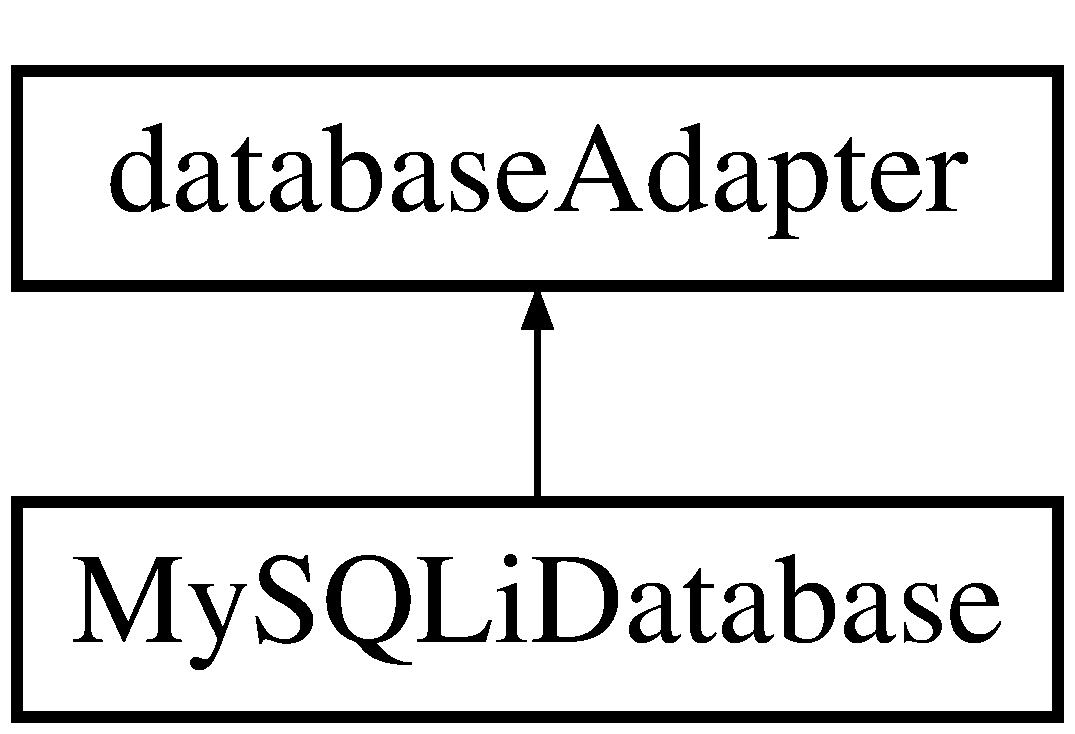
\includegraphics[height=2.000000cm]{class_my_s_q_li_database}
\end{center}
\end{figure}
\subsection*{Public Member Functions}
\begin{DoxyCompactItemize}
\item 
\hyperlink{class_my_s_q_li_database_a81fcddb424f13e0862ee3f7e1ea57ce9}{\_\-\_\-construct} (\$host, \$username, \$password, \$db)
\item 
\hyperlink{class_my_s_q_li_database_a4c4f3316747e665b9e02f6ddcba4117c}{connect} (\$host, \$username, \$password)
\item 
\hyperlink{class_my_s_q_li_database_abe175fcf658475bc56e9d6fa02bc88ec}{disconnect} ()
\item 
\hyperlink{class_my_s_q_li_database_a421831a265621325e1fdd19aace0c758}{\_\-\_\-destruct} ()
\item 
\hyperlink{class_my_s_q_li_database_ab624b0b234f9db9dbc6dc4180f566b1f}{selectDatabase} (\$db)
\item 
\hyperlink{class_my_s_q_li_database_a039ae2e8f2bf579fd75d9df8df87eee3}{escapeValue} (\$value)
\item 
\hyperlink{class_my_s_q_li_database_aebc962126fd37fd3478c4689156d5f83}{Query} (\$query)
\item 
\hyperlink{class_my_s_q_li_database_a3e35f6f5604ebbf57a86508c708bd33c}{fetchFirst} (\$query=false)
\item 
\hyperlink{class_my_s_q_li_database_acdee1c4e55c3792b3dbfeedfac35912f}{fetchRow} (\$query=false, \$type=1)
\item 
\hyperlink{class_my_s_q_li_database_a1750ab2493620de034b80a77577f3e8b}{fetchAll} (\$query=false, \$type=1)
\item 
\hyperlink{class_my_s_q_li_database_a24ada5decce3d1b79cd82f5a90ccf404}{getError} ()
\item 
\hyperlink{class_my_s_q_li_database_ac73f1d8cddbdfc35ca442189378a073c}{getInsertID} ()
\item 
\hyperlink{class_my_s_q_li_database_af37433a300db1f607ee789d22828a0a0}{numRows} ()
\item 
\hyperlink{class_my_s_q_li_database_acac8dfe61e7840f9a1e672ebede0be21}{numAffected} ()
\item 
\hyperlink{class_my_s_q_li_database_ae7cdaa744d52a1eb0103e377023ca528}{tableExists} (\$\hyperlink{classtable}{table})
\item 
\hyperlink{class_my_s_q_li_database_a4b06dfe3bf7dd552f828a80fece817d8}{createTable} (\$name, \$params)
\item 
\hyperlink{class_my_s_q_li_database_a3471d37afdd3d76f5379dfe7364db0b6}{dropTable} (\$name)
\item 
\hyperlink{class_my_s_q_li_database_aa8cf3e2be109e548bed6980622fffb41}{alterTable} (\$name, \$params)
\end{DoxyCompactItemize}
\subsection*{Data Fields}
\begin{DoxyCompactItemize}
\item 
\hyperlink{class_my_s_q_li_database_a0d9c79b9b86b3f5891c6d3892f12c6a0}{\$connection}
\item 
\hyperlink{class_my_s_q_li_database_a112ef069ddc0454086e3d1e6d8d55d07}{\$result}
\item 
\hyperlink{class_my_s_q_li_database_a7691c0162d89de0b6ba47edcd8ba8878}{\$database}
\item 
\hyperlink{class_my_s_q_li_database_a576b05de2f452e4cce4e3de12667ba0f}{\$queries}
\end{DoxyCompactItemize}


\subsection{Detailed Description}
MySQLi specific implementation of \hyperlink{interfacedatabase_adapter}{databaseAdapter} 

\subsection{Constructor \& Destructor Documentation}
\hypertarget{class_my_s_q_li_database_a81fcddb424f13e0862ee3f7e1ea57ce9}{
\index{MySQLiDatabase@{MySQLiDatabase}!\_\-\_\-construct@{\_\-\_\-construct}}
\index{\_\-\_\-construct@{\_\-\_\-construct}!MySQLiDatabase@{MySQLiDatabase}}
\subsubsection[{\_\-\_\-construct}]{\setlength{\rightskip}{0pt plus 5cm}\_\-\_\-construct (
\begin{DoxyParamCaption}
\item[{\$}]{host, }
\item[{\$}]{username, }
\item[{\$}]{password, }
\item[{\$}]{db}
\end{DoxyParamCaption}
)}}
\label{class_my_s_q_li_database_a81fcddb424f13e0862ee3f7e1ea57ce9}
Class constructor, initializes connection to MySQL database. Not implemented as singleton pattern because you can have connections to different databases. 
\begin{DoxyParams}[1]{Parameters}
string & {\em \$host} & \\
\hline
string & {\em \$username} & \\
\hline
string & {\em \$password} & \\
\hline
string & {\em \$db} & \\
\hline
\end{DoxyParams}


Reimplemented from \hyperlink{interfacedatabase_adapter_a81fcddb424f13e0862ee3f7e1ea57ce9}{databaseAdapter}.

\hypertarget{class_my_s_q_li_database_a421831a265621325e1fdd19aace0c758}{
\index{MySQLiDatabase@{MySQLiDatabase}!\_\-\_\-destruct@{\_\-\_\-destruct}}
\index{\_\-\_\-destruct@{\_\-\_\-destruct}!MySQLiDatabase@{MySQLiDatabase}}
\subsubsection[{\_\-\_\-destruct}]{\setlength{\rightskip}{0pt plus 5cm}\_\-\_\-destruct (
\begin{DoxyParamCaption}
{}
\end{DoxyParamCaption}
)}}
\label{class_my_s_q_li_database_a421831a265621325e1fdd19aace0c758}
Destructor of class. Disconnects from database. 

\subsection{Member Function Documentation}
\hypertarget{class_my_s_q_li_database_aa8cf3e2be109e548bed6980622fffb41}{
\index{MySQLiDatabase@{MySQLiDatabase}!alterTable@{alterTable}}
\index{alterTable@{alterTable}!MySQLiDatabase@{MySQLiDatabase}}
\subsubsection[{alterTable}]{\setlength{\rightskip}{0pt plus 5cm}alterTable (
\begin{DoxyParamCaption}
\item[{\$}]{name, }
\item[{\$}]{params}
\end{DoxyParamCaption}
)}}
\label{class_my_s_q_li_database_aa8cf3e2be109e548bed6980622fffb41}
Alters \$name table. To change it's name by \$params must containt an element with key 'name' and value the new name of the table in params. To add a column, \$paramas must contain an element with key 'add' and value an array of columns you wish to add (specified as at createTable. To modify a column, \$params must contain an element with key 'edit' and value an array of columns you wish to edit (specified as at createTable. To drop a column, \$params must contain an \$element with key 'delete' and value the name of the column you want to delete. 
\begin{DoxyParams}[1]{Parameters}
string & {\em \$name} & \\
\hline
array & {\em \$params} & \\
\hline
\end{DoxyParams}

\begin{DoxyRetVals}{Return values}
{\em true} & \\
\hline
{\em false} & \\
\hline
\end{DoxyRetVals}
\begin{Desc}
\item[\hyperlink{todo__todo000004}{Todo}]some checks for valid column names and parameters \end{Desc}


Reimplemented from \hyperlink{interfacedatabase_adapter_aa8cf3e2be109e548bed6980622fffb41}{databaseAdapter}.

\hypertarget{class_my_s_q_li_database_a4c4f3316747e665b9e02f6ddcba4117c}{
\index{MySQLiDatabase@{MySQLiDatabase}!connect@{connect}}
\index{connect@{connect}!MySQLiDatabase@{MySQLiDatabase}}
\subsubsection[{connect}]{\setlength{\rightskip}{0pt plus 5cm}connect (
\begin{DoxyParamCaption}
\item[{\$}]{host, }
\item[{\$}]{username, }
\item[{\$}]{password}
\end{DoxyParamCaption}
)}}
\label{class_my_s_q_li_database_a4c4f3316747e665b9e02f6ddcba4117c}


Reimplemented from \hyperlink{interfacedatabase_adapter_a4c4f3316747e665b9e02f6ddcba4117c}{databaseAdapter}.

\hypertarget{class_my_s_q_li_database_a4b06dfe3bf7dd552f828a80fece817d8}{
\index{MySQLiDatabase@{MySQLiDatabase}!createTable@{createTable}}
\index{createTable@{createTable}!MySQLiDatabase@{MySQLiDatabase}}
\subsubsection[{createTable}]{\setlength{\rightskip}{0pt plus 5cm}createTable (
\begin{DoxyParamCaption}
\item[{\$}]{name, }
\item[{\$}]{params}
\end{DoxyParamCaption}
)}}
\label{class_my_s_q_li_database_a4b06dfe3bf7dd552f828a80fece817d8}
Creates a table. 
\begin{DoxyParams}[1]{Parameters}
string & {\em \$name} & Has to match this regex \mbox{[}A-\/Za-\/z0-\/9\_\-\mbox{]}$\ast$ \\
\hline
array & {\em \$params} & Example: array('id'=$>$array('INT','NOT NULL','AUTO\_\-INCREMENT','PRIMARY KEY'),'text'=$>$array('TEXT','NOT NULL')) \\
\hline
\end{DoxyParams}

\begin{DoxyRetVals}{Return values}
{\em true} & \\
\hline
{\em false} & \\
\hline
\end{DoxyRetVals}


Reimplemented from \hyperlink{interfacedatabase_adapter_a4b06dfe3bf7dd552f828a80fece817d8}{databaseAdapter}.

\hypertarget{class_my_s_q_li_database_abe175fcf658475bc56e9d6fa02bc88ec}{
\index{MySQLiDatabase@{MySQLiDatabase}!disconnect@{disconnect}}
\index{disconnect@{disconnect}!MySQLiDatabase@{MySQLiDatabase}}
\subsubsection[{disconnect}]{\setlength{\rightskip}{0pt plus 5cm}disconnect (
\begin{DoxyParamCaption}
{}
\end{DoxyParamCaption}
)}}
\label{class_my_s_q_li_database_abe175fcf658475bc56e9d6fa02bc88ec}
Disconnects from the database 

Reimplemented from \hyperlink{interfacedatabase_adapter_abe175fcf658475bc56e9d6fa02bc88ec}{databaseAdapter}.

\hypertarget{class_my_s_q_li_database_a3471d37afdd3d76f5379dfe7364db0b6}{
\index{MySQLiDatabase@{MySQLiDatabase}!dropTable@{dropTable}}
\index{dropTable@{dropTable}!MySQLiDatabase@{MySQLiDatabase}}
\subsubsection[{dropTable}]{\setlength{\rightskip}{0pt plus 5cm}dropTable (
\begin{DoxyParamCaption}
\item[{\$}]{name}
\end{DoxyParamCaption}
)}}
\label{class_my_s_q_li_database_a3471d37afdd3d76f5379dfe7364db0b6}
It drops \$name table if it exists. If it doesn't exist it returns true (you wanted it gone, right?). 
\begin{DoxyParams}[1]{Parameters}
string & {\em \$name} & \\
\hline
\end{DoxyParams}

\begin{DoxyRetVals}{Return values}
{\em true} & \\
\hline
{\em false} & \\
\hline
\end{DoxyRetVals}


Reimplemented from \hyperlink{interfacedatabase_adapter_a3471d37afdd3d76f5379dfe7364db0b6}{databaseAdapter}.

\hypertarget{class_my_s_q_li_database_a039ae2e8f2bf579fd75d9df8df87eee3}{
\index{MySQLiDatabase@{MySQLiDatabase}!escapeValue@{escapeValue}}
\index{escapeValue@{escapeValue}!MySQLiDatabase@{MySQLiDatabase}}
\subsubsection[{escapeValue}]{\setlength{\rightskip}{0pt plus 5cm}escapeValue (
\begin{DoxyParamCaption}
\item[{\$}]{value}
\end{DoxyParamCaption}
)}}
\label{class_my_s_q_li_database_a039ae2e8f2bf579fd75d9df8df87eee3}
Escapes a string for safe MySQL insertion 
\begin{DoxyParams}[1]{Parameters}
string & {\em \$value} & \\
\hline
\end{DoxyParams}
\begin{DoxyReturn}{Returns}
string 
\end{DoxyReturn}


Reimplemented from \hyperlink{interfacedatabase_adapter_a039ae2e8f2bf579fd75d9df8df87eee3}{databaseAdapter}.

\hypertarget{class_my_s_q_li_database_a1750ab2493620de034b80a77577f3e8b}{
\index{MySQLiDatabase@{MySQLiDatabase}!fetchAll@{fetchAll}}
\index{fetchAll@{fetchAll}!MySQLiDatabase@{MySQLiDatabase}}
\subsubsection[{fetchAll}]{\setlength{\rightskip}{0pt plus 5cm}fetchAll (
\begin{DoxyParamCaption}
\item[{\$}]{query = {\ttfamily false}, }
\item[{\$}]{type = {\ttfamily 1}}
\end{DoxyParamCaption}
)}}
\label{class_my_s_q_li_database_a1750ab2493620de034b80a77577f3e8b}
Fetches all the rows from the results of a query. Returns numeric array, associative array or both depending on second parameter:1,2,3 
\begin{DoxyParams}[1]{Parameters}
string & {\em \$query} & \\
\hline
int & {\em \$type} & 1 -\/ Associative array, 2 -\/ Numeric array, 3 -\/ Both \\
\hline
\end{DoxyParams}
\begin{DoxyReturn}{Returns}
mixed 
\end{DoxyReturn}


Reimplemented from \hyperlink{interfacedatabase_adapter_a861f65695740a1d866ce1001f0ae706d}{databaseAdapter}.

\hypertarget{class_my_s_q_li_database_a3e35f6f5604ebbf57a86508c708bd33c}{
\index{MySQLiDatabase@{MySQLiDatabase}!fetchFirst@{fetchFirst}}
\index{fetchFirst@{fetchFirst}!MySQLiDatabase@{MySQLiDatabase}}
\subsubsection[{fetchFirst}]{\setlength{\rightskip}{0pt plus 5cm}fetchFirst (
\begin{DoxyParamCaption}
\item[{\$}]{query = {\ttfamily false}}
\end{DoxyParamCaption}
)}}
\label{class_my_s_q_li_database_a3e35f6f5604ebbf57a86508c708bd33c}
Fetches the first value from the first row. 
\begin{DoxyParams}[1]{Parameters}
string & {\em \$query} & \\
\hline
\end{DoxyParams}
\begin{DoxyReturn}{Returns}
mixed 
\end{DoxyReturn}
\hypertarget{class_my_s_q_li_database_acdee1c4e55c3792b3dbfeedfac35912f}{
\index{MySQLiDatabase@{MySQLiDatabase}!fetchRow@{fetchRow}}
\index{fetchRow@{fetchRow}!MySQLiDatabase@{MySQLiDatabase}}
\subsubsection[{fetchRow}]{\setlength{\rightskip}{0pt plus 5cm}fetchRow (
\begin{DoxyParamCaption}
\item[{\$}]{query = {\ttfamily false}, }
\item[{\$}]{type = {\ttfamily 1}}
\end{DoxyParamCaption}
)}}
\label{class_my_s_q_li_database_acdee1c4e55c3792b3dbfeedfac35912f}
Fetches first row from the results of a query. Returns numeric array, associative array or both depending on second parameter:1,2,3 
\begin{DoxyParams}[1]{Parameters}
string & {\em \$query} & \\
\hline
int & {\em \$type} & 1 -\/ Associative array, 2 -\/ Numeric array, 3 -\/ Both \\
\hline
\end{DoxyParams}
\begin{DoxyReturn}{Returns}
mixed 
\end{DoxyReturn}


Reimplemented from \hyperlink{interfacedatabase_adapter_a529385852efa66f19288496930ee5394}{databaseAdapter}.

\hypertarget{class_my_s_q_li_database_a24ada5decce3d1b79cd82f5a90ccf404}{
\index{MySQLiDatabase@{MySQLiDatabase}!getError@{getError}}
\index{getError@{getError}!MySQLiDatabase@{MySQLiDatabase}}
\subsubsection[{getError}]{\setlength{\rightskip}{0pt plus 5cm}getError (
\begin{DoxyParamCaption}
{}
\end{DoxyParamCaption}
)}}
\label{class_my_s_q_li_database_a24ada5decce3d1b79cd82f5a90ccf404}
Return the last MySQLi error \begin{DoxyReturn}{Returns}
string 
\end{DoxyReturn}


Reimplemented from \hyperlink{interfacedatabase_adapter_a24ada5decce3d1b79cd82f5a90ccf404}{databaseAdapter}.

\hypertarget{class_my_s_q_li_database_ac73f1d8cddbdfc35ca442189378a073c}{
\index{MySQLiDatabase@{MySQLiDatabase}!getInsertID@{getInsertID}}
\index{getInsertID@{getInsertID}!MySQLiDatabase@{MySQLiDatabase}}
\subsubsection[{getInsertID}]{\setlength{\rightskip}{0pt plus 5cm}getInsertID (
\begin{DoxyParamCaption}
{}
\end{DoxyParamCaption}
)}}
\label{class_my_s_q_li_database_ac73f1d8cddbdfc35ca442189378a073c}
Returns the id of the last insertion \begin{DoxyReturn}{Returns}
int 
\end{DoxyReturn}


Reimplemented from \hyperlink{interfacedatabase_adapter_ac73f1d8cddbdfc35ca442189378a073c}{databaseAdapter}.

\hypertarget{class_my_s_q_li_database_acac8dfe61e7840f9a1e672ebede0be21}{
\index{MySQLiDatabase@{MySQLiDatabase}!numAffected@{numAffected}}
\index{numAffected@{numAffected}!MySQLiDatabase@{MySQLiDatabase}}
\subsubsection[{numAffected}]{\setlength{\rightskip}{0pt plus 5cm}numAffected (
\begin{DoxyParamCaption}
{}
\end{DoxyParamCaption}
)}}
\label{class_my_s_q_li_database_acac8dfe61e7840f9a1e672ebede0be21}
Returns the number of rows affected by an UPDATE query \begin{DoxyReturn}{Returns}
int 
\end{DoxyReturn}


Reimplemented from \hyperlink{interfacedatabase_adapter_acac8dfe61e7840f9a1e672ebede0be21}{databaseAdapter}.

\hypertarget{class_my_s_q_li_database_af37433a300db1f607ee789d22828a0a0}{
\index{MySQLiDatabase@{MySQLiDatabase}!numRows@{numRows}}
\index{numRows@{numRows}!MySQLiDatabase@{MySQLiDatabase}}
\subsubsection[{numRows}]{\setlength{\rightskip}{0pt plus 5cm}numRows (
\begin{DoxyParamCaption}
{}
\end{DoxyParamCaption}
)}}
\label{class_my_s_q_li_database_af37433a300db1f607ee789d22828a0a0}
Returns the number of rows from a query \begin{DoxyReturn}{Returns}
int 
\end{DoxyReturn}


Reimplemented from \hyperlink{interfacedatabase_adapter_af37433a300db1f607ee789d22828a0a0}{databaseAdapter}.

\hypertarget{class_my_s_q_li_database_aebc962126fd37fd3478c4689156d5f83}{
\index{MySQLiDatabase@{MySQLiDatabase}!Query@{Query}}
\index{Query@{Query}!MySQLiDatabase@{MySQLiDatabase}}
\subsubsection[{Query}]{\setlength{\rightskip}{0pt plus 5cm}{\bf Query} (
\begin{DoxyParamCaption}
\item[{\$}]{query}
\end{DoxyParamCaption}
)}}
\label{class_my_s_q_li_database_aebc962126fd37fd3478c4689156d5f83}
Executes query 
\begin{DoxyParams}[1]{Parameters}
string & {\em \$query} & \\
\hline
\end{DoxyParams}
\begin{DoxyReturn}{Returns}
mixed 
\end{DoxyReturn}
\begin{Desc}
\item[\hyperlink{todo__todo000003}{Todo}]change return values for insert, update, delete, select \end{Desc}
\hypertarget{class_my_s_q_li_database_ab624b0b234f9db9dbc6dc4180f566b1f}{
\index{MySQLiDatabase@{MySQLiDatabase}!selectDatabase@{selectDatabase}}
\index{selectDatabase@{selectDatabase}!MySQLiDatabase@{MySQLiDatabase}}
\subsubsection[{selectDatabase}]{\setlength{\rightskip}{0pt plus 5cm}selectDatabase (
\begin{DoxyParamCaption}
\item[{\$}]{db}
\end{DoxyParamCaption}
)}}
\label{class_my_s_q_li_database_ab624b0b234f9db9dbc6dc4180f566b1f}
Connects to a different database 
\begin{DoxyParams}[1]{Parameters}
string & {\em \$db} & \\
\hline
\end{DoxyParams}

\begin{DoxyRetVals}{Return values}
{\em true} & \\
\hline
{\em false} & \\
\hline
\end{DoxyRetVals}


Reimplemented from \hyperlink{interfacedatabase_adapter_ab624b0b234f9db9dbc6dc4180f566b1f}{databaseAdapter}.

\hypertarget{class_my_s_q_li_database_ae7cdaa744d52a1eb0103e377023ca528}{
\index{MySQLiDatabase@{MySQLiDatabase}!tableExists@{tableExists}}
\index{tableExists@{tableExists}!MySQLiDatabase@{MySQLiDatabase}}
\subsubsection[{tableExists}]{\setlength{\rightskip}{0pt plus 5cm}tableExists (
\begin{DoxyParamCaption}
\item[{\$}]{table}
\end{DoxyParamCaption}
)}}
\label{class_my_s_q_li_database_ae7cdaa744d52a1eb0103e377023ca528}
Checks if a table exists 
\begin{DoxyParams}[1]{Parameters}
string & {\em \$table} & \\
\hline
\end{DoxyParams}

\begin{DoxyRetVals}{Return values}
{\em true} & \\
\hline
{\em false} & \\
\hline
\end{DoxyRetVals}


Reimplemented from \hyperlink{interfacedatabase_adapter_ae7cdaa744d52a1eb0103e377023ca528}{databaseAdapter}.



\subsection{Field Documentation}
\hypertarget{class_my_s_q_li_database_a0d9c79b9b86b3f5891c6d3892f12c6a0}{
\index{MySQLiDatabase@{MySQLiDatabase}!\$connection@{\$connection}}
\index{\$connection@{\$connection}!MySQLiDatabase@{MySQLiDatabase}}
\subsubsection[{\$connection}]{\setlength{\rightskip}{0pt plus 5cm}\$connection}}
\label{class_my_s_q_li_database_a0d9c79b9b86b3f5891c6d3892f12c6a0}
Stores the MySQLi connection \hypertarget{class_my_s_q_li_database_a7691c0162d89de0b6ba47edcd8ba8878}{
\index{MySQLiDatabase@{MySQLiDatabase}!\$database@{\$database}}
\index{\$database@{\$database}!MySQLiDatabase@{MySQLiDatabase}}
\subsubsection[{\$database}]{\setlength{\rightskip}{0pt plus 5cm}\$database}}
\label{class_my_s_q_li_database_a7691c0162d89de0b6ba47edcd8ba8878}
Stores the working database \hypertarget{class_my_s_q_li_database_a576b05de2f452e4cce4e3de12667ba0f}{
\index{MySQLiDatabase@{MySQLiDatabase}!\$queries@{\$queries}}
\index{\$queries@{\$queries}!MySQLiDatabase@{MySQLiDatabase}}
\subsubsection[{\$queries}]{\setlength{\rightskip}{0pt plus 5cm}\$queries}}
\label{class_my_s_q_li_database_a576b05de2f452e4cce4e3de12667ba0f}
Stores all the queries that have been executed \hypertarget{class_my_s_q_li_database_a112ef069ddc0454086e3d1e6d8d55d07}{
\index{MySQLiDatabase@{MySQLiDatabase}!\$result@{\$result}}
\index{\$result@{\$result}!MySQLiDatabase@{MySQLiDatabase}}
\subsubsection[{\$result}]{\setlength{\rightskip}{0pt plus 5cm}\$result}}
\label{class_my_s_q_li_database_a112ef069ddc0454086e3d1e6d8d55d07}
Stores the latest result from a query 

The documentation for this class was generated from the following file:\begin{DoxyCompactItemize}
\item 
C:/wamp/www/framework/\hyperlink{database_adapter_8php}{databaseAdapter.php}\end{DoxyCompactItemize}

\hypertarget{class_query}{
\section{Query Class Reference}
\label{class_query}\index{Query@{Query}}
}
Inheritance diagram for Query:\begin{figure}[H]
\begin{center}
\leavevmode
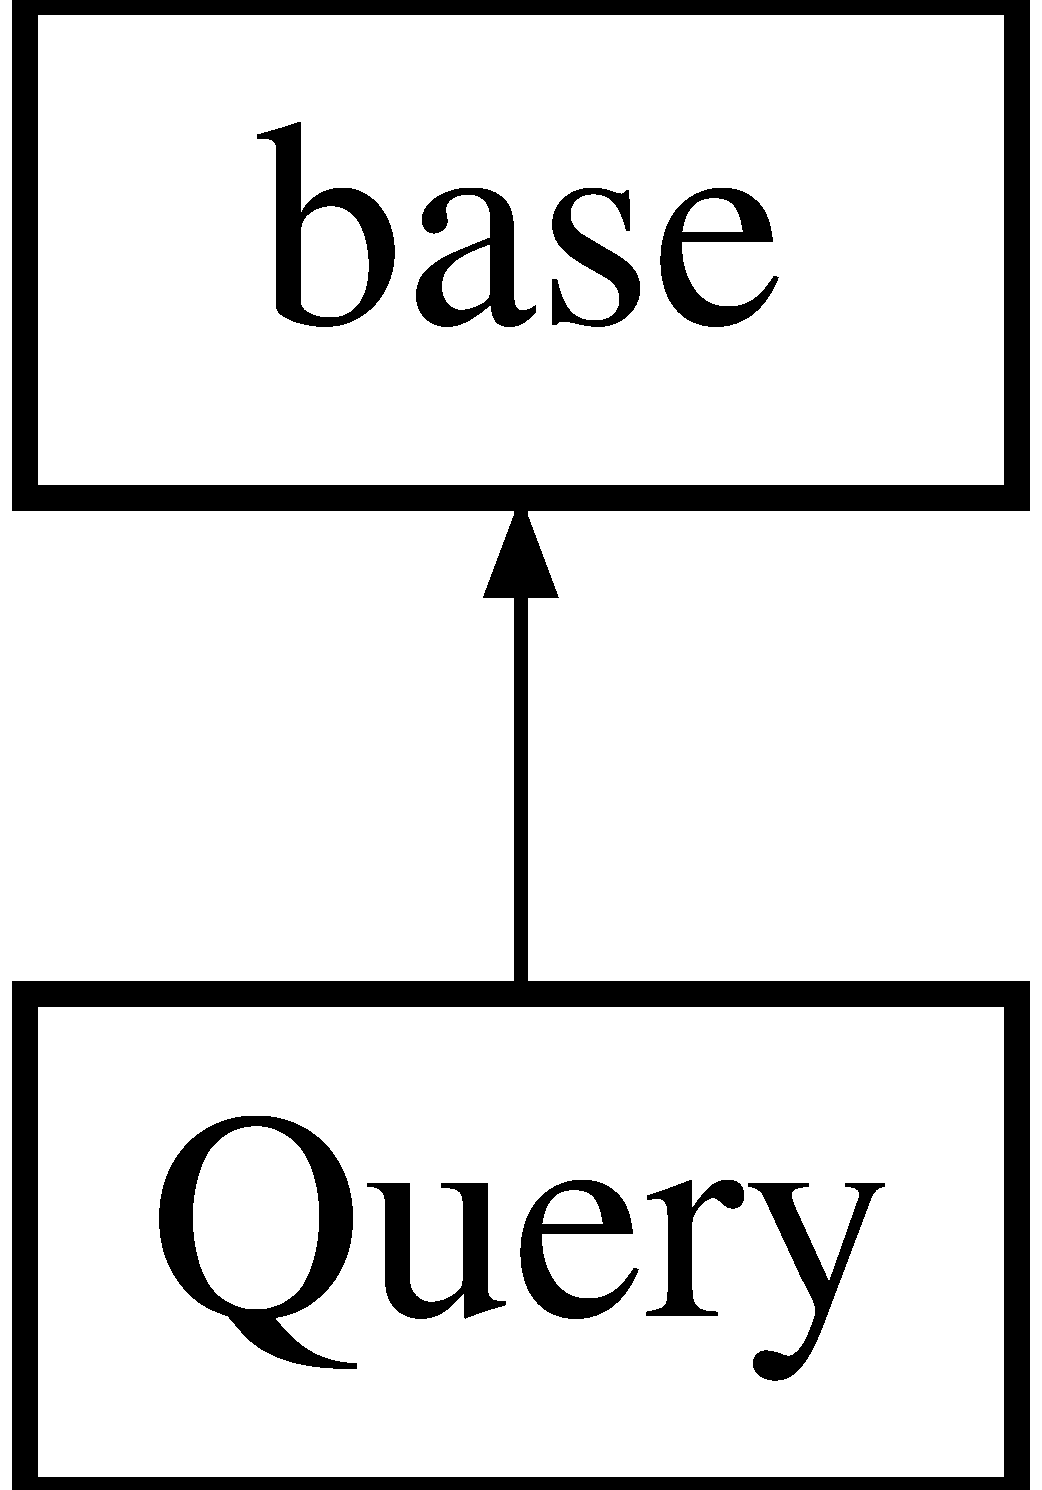
\includegraphics[height=2.000000cm]{class_query}
\end{center}
\end{figure}
\subsection*{Public Member Functions}
\begin{DoxyCompactItemize}
\item 
\hyperlink{class_query_a28e580fac4fbdedecd32b8ccb932b157}{\_\-\_\-construct} (\$class, \$filters, \$ordergroup, \$columns)
\item 
\hyperlink{class_query_a394445491b1b221e4e562dfb45f2a266}{buildQuery} ()
\item 
\hyperlink{class_query_a24d4dbc71552d9387256a3cc426e3898}{getCount} ()
\end{DoxyCompactItemize}


\subsection{Detailed Description}
/class \hyperlink{class_query}{Query} Helper class for making the more complicated queries. 

\subsection{Constructor \& Destructor Documentation}
\hypertarget{class_query_a28e580fac4fbdedecd32b8ccb932b157}{
\index{Query@{Query}!\_\-\_\-construct@{\_\-\_\-construct}}
\index{\_\-\_\-construct@{\_\-\_\-construct}!Query@{Query}}
\subsubsection[{\_\-\_\-construct}]{\setlength{\rightskip}{0pt plus 5cm}\_\-\_\-construct (
\begin{DoxyParamCaption}
\item[{\$}]{class, }
\item[{\$}]{filters, }
\item[{\$}]{ordergroup, }
\item[{\$}]{columns}
\end{DoxyParamCaption}
)}}
\label{class_query_a28e580fac4fbdedecd32b8ccb932b157}
Constructor. 
\begin{DoxyParams}[1]{Parameters}
string & {\em \$class} & \\
\hline
array & {\em \$filters} & \\
\hline
array & {\em \$ordergroup} & \\
\hline
array & {\em \$columns} & \\
\hline
\end{DoxyParams}


\subsection{Member Function Documentation}
\hypertarget{class_query_a394445491b1b221e4e562dfb45f2a266}{
\index{Query@{Query}!buildQuery@{buildQuery}}
\index{buildQuery@{buildQuery}!Query@{Query}}
\subsubsection[{buildQuery}]{\setlength{\rightskip}{0pt plus 5cm}buildQuery (
\begin{DoxyParamCaption}
{}
\end{DoxyParamCaption}
)}}
\label{class_query_a394445491b1b221e4e562dfb45f2a266}
Simply joins and returns all the stuff done in the previous functions \begin{DoxyReturn}{Returns}
string with SQL statement 
\end{DoxyReturn}
\hypertarget{class_query_a24d4dbc71552d9387256a3cc426e3898}{
\index{Query@{Query}!getCount@{getCount}}
\index{getCount@{getCount}!Query@{Query}}
\subsubsection[{getCount}]{\setlength{\rightskip}{0pt plus 5cm}getCount (
\begin{DoxyParamCaption}
{}
\end{DoxyParamCaption}
)}}
\label{class_query_a24d4dbc71552d9387256a3cc426e3898}
Get's a count for how many rows would a query return \begin{DoxyReturn}{Returns}
int; 
\end{DoxyReturn}


The documentation for this class was generated from the following file:\begin{DoxyCompactItemize}
\item 
C:/wamp/www/framework/\hyperlink{db_8php}{db.php}\end{DoxyCompactItemize}

\hypertarget{classrolisz}{
\section{rolisz Class Reference}
\label{classrolisz}\index{rolisz@{rolisz}}
}
Inheritance diagram for rolisz:\begin{figure}[H]
\begin{center}
\leavevmode
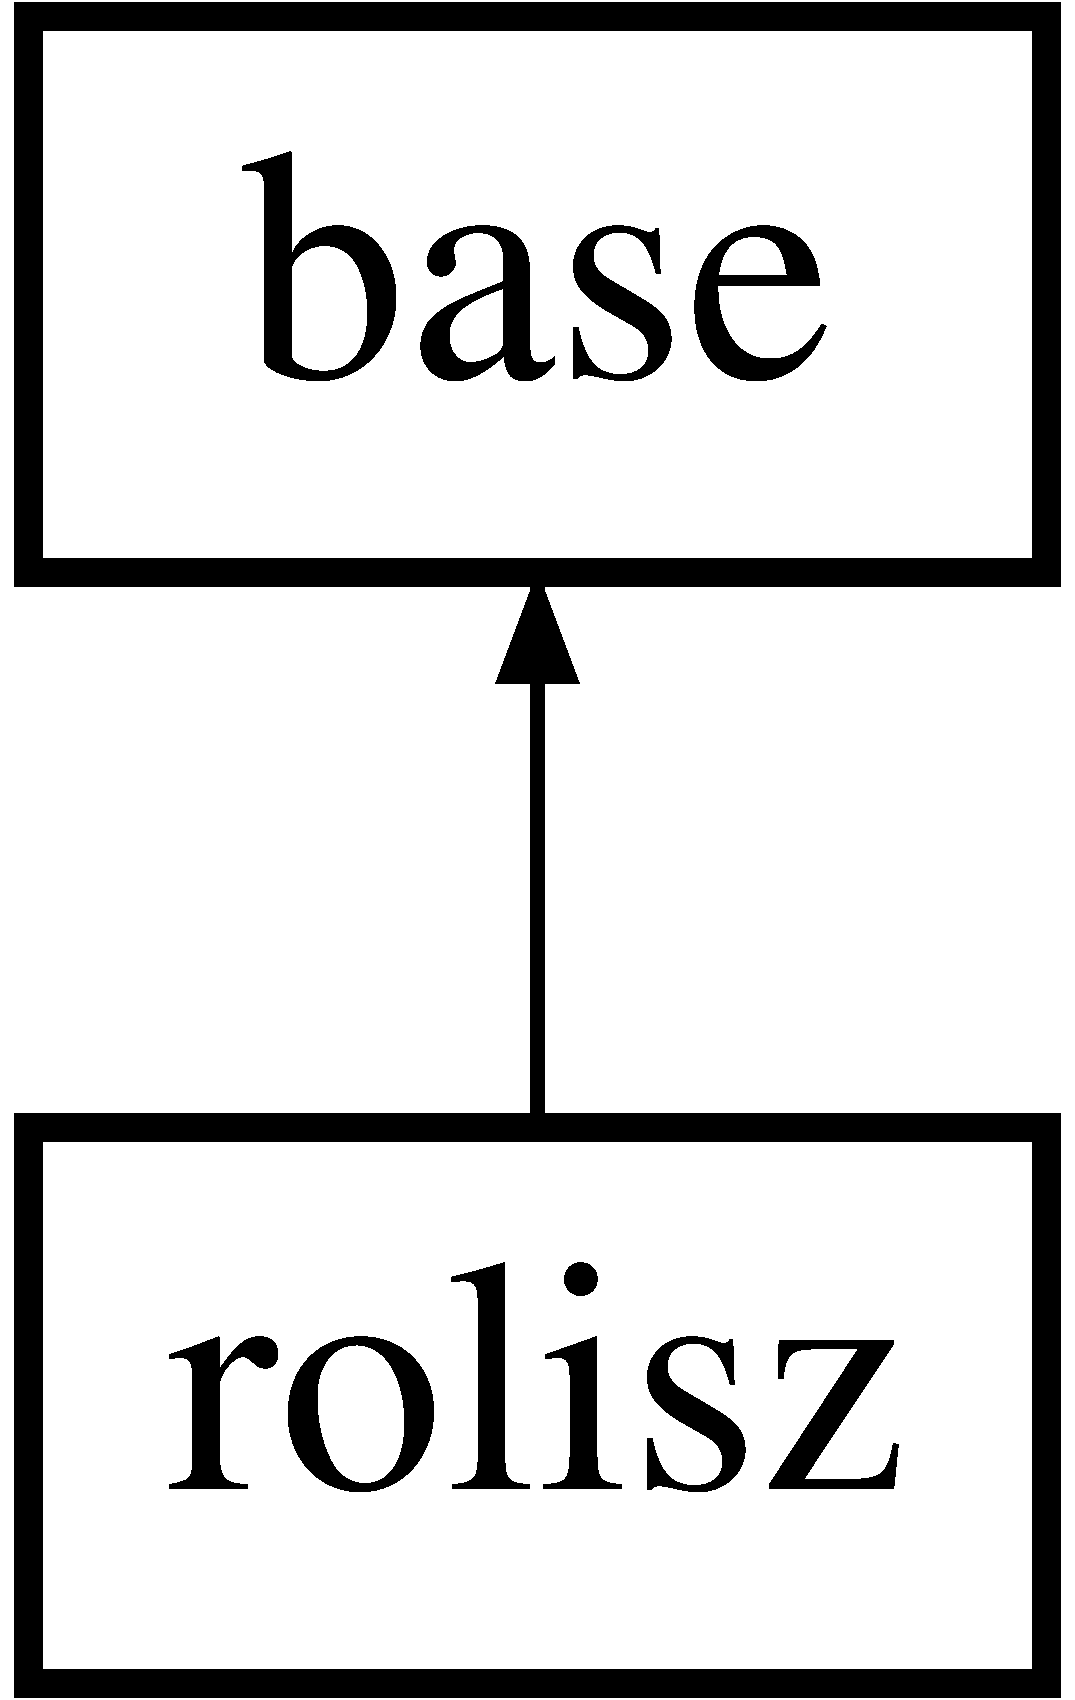
\includegraphics[height=2.000000cm]{classrolisz}
\end{center}
\end{figure}
\subsection*{Static Public Member Functions}
\begin{DoxyCompactItemize}
\item 
static \hyperlink{classrolisz_af732c33c326c863efe6dd2cccb21a9a5}{call} (\$funcs, \$args)
\item 
static \hyperlink{classrolisz_a7cee6d5c562bcb595bc9d826910d248d}{connect} (\$dbtype, \$host, \$username, \$password, \$db)
\item 
static \hyperlink{classrolisz_ab4c022bf9d3474583030f31894865182}{autoload} (\$class)
\item 
static \hyperlink{classrolisz_a6fdc4c9fc517c619d860c7e91d17b02d}{http404} ()
\item 
static \hyperlink{classrolisz_a13d0c0500b75a5bdd849a4a55ba8e2b1}{fixSlashes} (\$str)
\item 
static \hyperlink{classrolisz_a031dd360aea86d999059dbfd18687973}{fixQuotes} (\$val)
\item 
static \hyperlink{classrolisz_ab8e0e9e5ffd59108f38efefe79511c5b}{fixBraces} (\$str)
\item 
static \hyperlink{classrolisz_aafd29366ef6399da1dd079fc131d8858}{route} (\$pattern, \$funcs, \$http= 'GET', \$name=FALSE)
\item 
static \hyperlink{classrolisz_ad3a572002fd350672b531756f7306e8f}{run} ()
\item 
static \hyperlink{classrolisz_a2c24b81993e81c6401edd6c4caff0336}{urlFor} (\$name, \$params=array())
\item 
static \hyperlink{classrolisz_ac871964dd21bf398baa7f61ecea0b895}{table} (\$\hyperlink{classtable}{table}, \$id=FALSE, \$columns=FALSE, \$connection=FALSE)
\item 
static \hyperlink{classrolisz_a146085d0f3a9d17bdcd7f3d4081d8c0d}{start} ()
\end{DoxyCompactItemize}


\subsection{Detailed Description}
Central class, contains only general useful functions or wrappers for the other classes 

\subsection{Member Function Documentation}
\hypertarget{classrolisz_ab4c022bf9d3474583030f31894865182}{
\index{rolisz@{rolisz}!autoload@{autoload}}
\index{autoload@{autoload}!rolisz@{rolisz}}
\subsubsection[{autoload}]{\setlength{\rightskip}{0pt plus 5cm}static autoload (
\begin{DoxyParamCaption}
\item[{\$}]{class}
\end{DoxyParamCaption}
)\hspace{0.3cm}{\ttfamily  \mbox{[}static\mbox{]}}}}
\label{classrolisz_ab4c022bf9d3474583030f31894865182}
Autoloader function. Lazy-\/loads classes from files in the same directory as current one. Files must be named the same the classes 
\begin{DoxyParams}[1]{Parameters}
string & {\em \$class} & \\
\hline
\end{DoxyParams}
\hypertarget{classrolisz_af732c33c326c863efe6dd2cccb21a9a5}{
\index{rolisz@{rolisz}!call@{call}}
\index{call@{call}!rolisz@{rolisz}}
\subsubsection[{call}]{\setlength{\rightskip}{0pt plus 5cm}static call (
\begin{DoxyParamCaption}
\item[{\$}]{funcs, }
\item[{\$}]{args}
\end{DoxyParamCaption}
)\hspace{0.3cm}{\ttfamily  \mbox{[}static\mbox{]}}}}
\label{classrolisz_af732c33c326c863efe6dd2cccb21a9a5}
Provide sandbox for functions and import files to prevent direct access to framework internals and other scripts 
\begin{DoxyParams}[1]{Parameters}
mixed & {\em \$funcs} & \\
\hline
array & {\em \$args} & \\
\hline
\end{DoxyParams}
\hypertarget{classrolisz_a7cee6d5c562bcb595bc9d826910d248d}{
\index{rolisz@{rolisz}!connect@{connect}}
\index{connect@{connect}!rolisz@{rolisz}}
\subsubsection[{connect}]{\setlength{\rightskip}{0pt plus 5cm}static connect (
\begin{DoxyParamCaption}
\item[{\$}]{dbtype, }
\item[{\$}]{host, }
\item[{\$}]{username, }
\item[{\$}]{password, }
\item[{\$}]{db}
\end{DoxyParamCaption}
)\hspace{0.3cm}{\ttfamily  \mbox{[}static\mbox{]}}}}
\label{classrolisz_a7cee6d5c562bcb595bc9d826910d248d}
Connects to a database adapter that implements the interface defined in \hyperlink{database_adapter_8php}{databaseAdapter.php} Checks for the existence of the class in \hyperlink{database_adapter_8php}{databaseAdapter.php} and a file called \$dbtype.DatabaseAdapter.php 
\begin{DoxyParams}[1]{Parameters}
string & {\em \$dbtype} & Database type. For now there is support for MySQL \\
\hline
string & {\em \$host} & \\
\hline
string & {\em \$username} & \\
\hline
string & {\em \$password} & \\
\hline
string & {\em \$db} & \\
\hline
\end{DoxyParams}
\begin{DoxyReturn}{Returns}
\hyperlink{interfacedatabase_adapter}{databaseAdapter} 
\end{DoxyReturn}
\hypertarget{classrolisz_ab8e0e9e5ffd59108f38efefe79511c5b}{
\index{rolisz@{rolisz}!fixBraces@{fixBraces}}
\index{fixBraces@{fixBraces}!rolisz@{rolisz}}
\subsubsection[{fixBraces}]{\setlength{\rightskip}{0pt plus 5cm}static fixBraces (
\begin{DoxyParamCaption}
\item[{\$}]{str}
\end{DoxyParamCaption}
)\hspace{0.3cm}{\ttfamily  \mbox{[}static\mbox{]}}}}
\label{classrolisz_ab8e0e9e5ffd59108f38efefe79511c5b}
Fix mangled braces 
\begin{DoxyParams}[1]{Parameters}
string & {\em \$str} & \\
\hline
\end{DoxyParams}
\begin{DoxyReturn}{Returns}
string 
\end{DoxyReturn}
\hypertarget{classrolisz_a031dd360aea86d999059dbfd18687973}{
\index{rolisz@{rolisz}!fixQuotes@{fixQuotes}}
\index{fixQuotes@{fixQuotes}!rolisz@{rolisz}}
\subsubsection[{fixQuotes}]{\setlength{\rightskip}{0pt plus 5cm}static fixQuotes (
\begin{DoxyParamCaption}
\item[{\$}]{val}
\end{DoxyParamCaption}
)\hspace{0.3cm}{\ttfamily  \mbox{[}static\mbox{]}}}}
\label{classrolisz_a031dd360aea86d999059dbfd18687973}
Convert double quotes to equivalent XML entities (\&\#34;) 
\begin{DoxyParams}[1]{Parameters}
string & {\em \$val} & \\
\hline
\end{DoxyParams}
\begin{DoxyReturn}{Returns}
string 
\end{DoxyReturn}
\hypertarget{classrolisz_a13d0c0500b75a5bdd849a4a55ba8e2b1}{
\index{rolisz@{rolisz}!fixSlashes@{fixSlashes}}
\index{fixSlashes@{fixSlashes}!rolisz@{rolisz}}
\subsubsection[{fixSlashes}]{\setlength{\rightskip}{0pt plus 5cm}static fixSlashes (
\begin{DoxyParamCaption}
\item[{\$}]{str}
\end{DoxyParamCaption}
)\hspace{0.3cm}{\ttfamily  \mbox{[}static\mbox{]}}}}
\label{classrolisz_a13d0c0500b75a5bdd849a4a55ba8e2b1}
Convert Windows double-\/backslashes to slashes 
\begin{DoxyParams}[1]{Parameters}
string & {\em \$str} & \\
\hline
\end{DoxyParams}
\begin{DoxyReturn}{Returns}
string 
\end{DoxyReturn}
\hypertarget{classrolisz_a6fdc4c9fc517c619d860c7e91d17b02d}{
\index{rolisz@{rolisz}!http404@{http404}}
\index{http404@{http404}!rolisz@{rolisz}}
\subsubsection[{http404}]{\setlength{\rightskip}{0pt plus 5cm}static http404 (
\begin{DoxyParamCaption}
{}
\end{DoxyParamCaption}
)\hspace{0.3cm}{\ttfamily  \mbox{[}static\mbox{]}}}}
\label{classrolisz_a6fdc4c9fc517c619d860c7e91d17b02d}
Trigger an HTTP 404 error. If the 404 framework variable has been set to a function, it will get called. Else, it just triggers an error saying the page was not found. \hypertarget{classrolisz_aafd29366ef6399da1dd079fc131d8858}{
\index{rolisz@{rolisz}!route@{route}}
\index{route@{route}!rolisz@{rolisz}}
\subsubsection[{route}]{\setlength{\rightskip}{0pt plus 5cm}static route (
\begin{DoxyParamCaption}
\item[{\$}]{pattern, }
\item[{\$}]{funcs, }
\item[{\$}]{http = {\ttfamily 'GET'}, }
\item[{\$}]{name = {\ttfamily FALSE}}
\end{DoxyParamCaption}
)\hspace{0.3cm}{\ttfamily  \mbox{[}static\mbox{]}}}}
\label{classrolisz_aafd29366ef6399da1dd079fc131d8858}
Wrappers for the router class \begin{DoxySeeAlso}{See also}
\hyperlink{classrouter_aafd29366ef6399da1dd079fc131d8858}{router::route} 
\end{DoxySeeAlso}
\hypertarget{classrolisz_ad3a572002fd350672b531756f7306e8f}{
\index{rolisz@{rolisz}!run@{run}}
\index{run@{run}!rolisz@{rolisz}}
\subsubsection[{run}]{\setlength{\rightskip}{0pt plus 5cm}static run (
\begin{DoxyParamCaption}
{}
\end{DoxyParamCaption}
)\hspace{0.3cm}{\ttfamily  \mbox{[}static\mbox{]}}}}
\label{classrolisz_ad3a572002fd350672b531756f7306e8f}
\begin{DoxySeeAlso}{See also}
\hyperlink{classrouter_ad3a572002fd350672b531756f7306e8f}{router::run} 
\end{DoxySeeAlso}
\hypertarget{classrolisz_a146085d0f3a9d17bdcd7f3d4081d8c0d}{
\index{rolisz@{rolisz}!start@{start}}
\index{start@{start}!rolisz@{rolisz}}
\subsubsection[{start}]{\setlength{\rightskip}{0pt plus 5cm}static start (
\begin{DoxyParamCaption}
{}
\end{DoxyParamCaption}
)\hspace{0.3cm}{\ttfamily  \mbox{[}static\mbox{]}}}}
\label{classrolisz_a146085d0f3a9d17bdcd7f3d4081d8c0d}
Sets up autoload, initializes some constants. \hypertarget{classrolisz_ac871964dd21bf398baa7f61ecea0b895}{
\index{rolisz@{rolisz}!table@{table}}
\index{table@{table}!rolisz@{rolisz}}
\subsubsection[{table}]{\setlength{\rightskip}{0pt plus 5cm}static {\bf table} (
\begin{DoxyParamCaption}
\item[{\$}]{table, }
\item[{\$}]{id = {\ttfamily FALSE}, }
\item[{\$}]{columns = {\ttfamily FALSE}, }
\item[{\$}]{connection = {\ttfamily FALSE}}
\end{DoxyParamCaption}
)\hspace{0.3cm}{\ttfamily  \mbox{[}static\mbox{]}}}}
\label{classrolisz_ac871964dd21bf398baa7f61ecea0b895}
Wrappers for tables \begin{DoxySeeAlso}{See also}
\hyperlink{classtable}{table} 
\end{DoxySeeAlso}
\hypertarget{classrolisz_a2c24b81993e81c6401edd6c4caff0336}{
\index{rolisz@{rolisz}!urlFor@{urlFor}}
\index{urlFor@{urlFor}!rolisz@{rolisz}}
\subsubsection[{urlFor}]{\setlength{\rightskip}{0pt plus 5cm}static urlFor (
\begin{DoxyParamCaption}
\item[{\$}]{name, }
\item[{\$}]{params = {\ttfamily array()}}
\end{DoxyParamCaption}
)\hspace{0.3cm}{\ttfamily  \mbox{[}static\mbox{]}}}}
\label{classrolisz_a2c24b81993e81c6401edd6c4caff0336}
\begin{DoxySeeAlso}{See also}
\hyperlink{classrouter_a2c24b81993e81c6401edd6c4caff0336}{router::urlFor} 
\end{DoxySeeAlso}


The documentation for this class was generated from the following file:\begin{DoxyCompactItemize}
\item 
C:/wamp/www/framework/\hyperlink{rolisz_8php}{rolisz.php}\end{DoxyCompactItemize}

\hypertarget{classrouter}{
\section{router Class Reference}
\label{classrouter}\index{router@{router}}
}
Inheritance diagram for router:\begin{figure}[H]
\begin{center}
\leavevmode
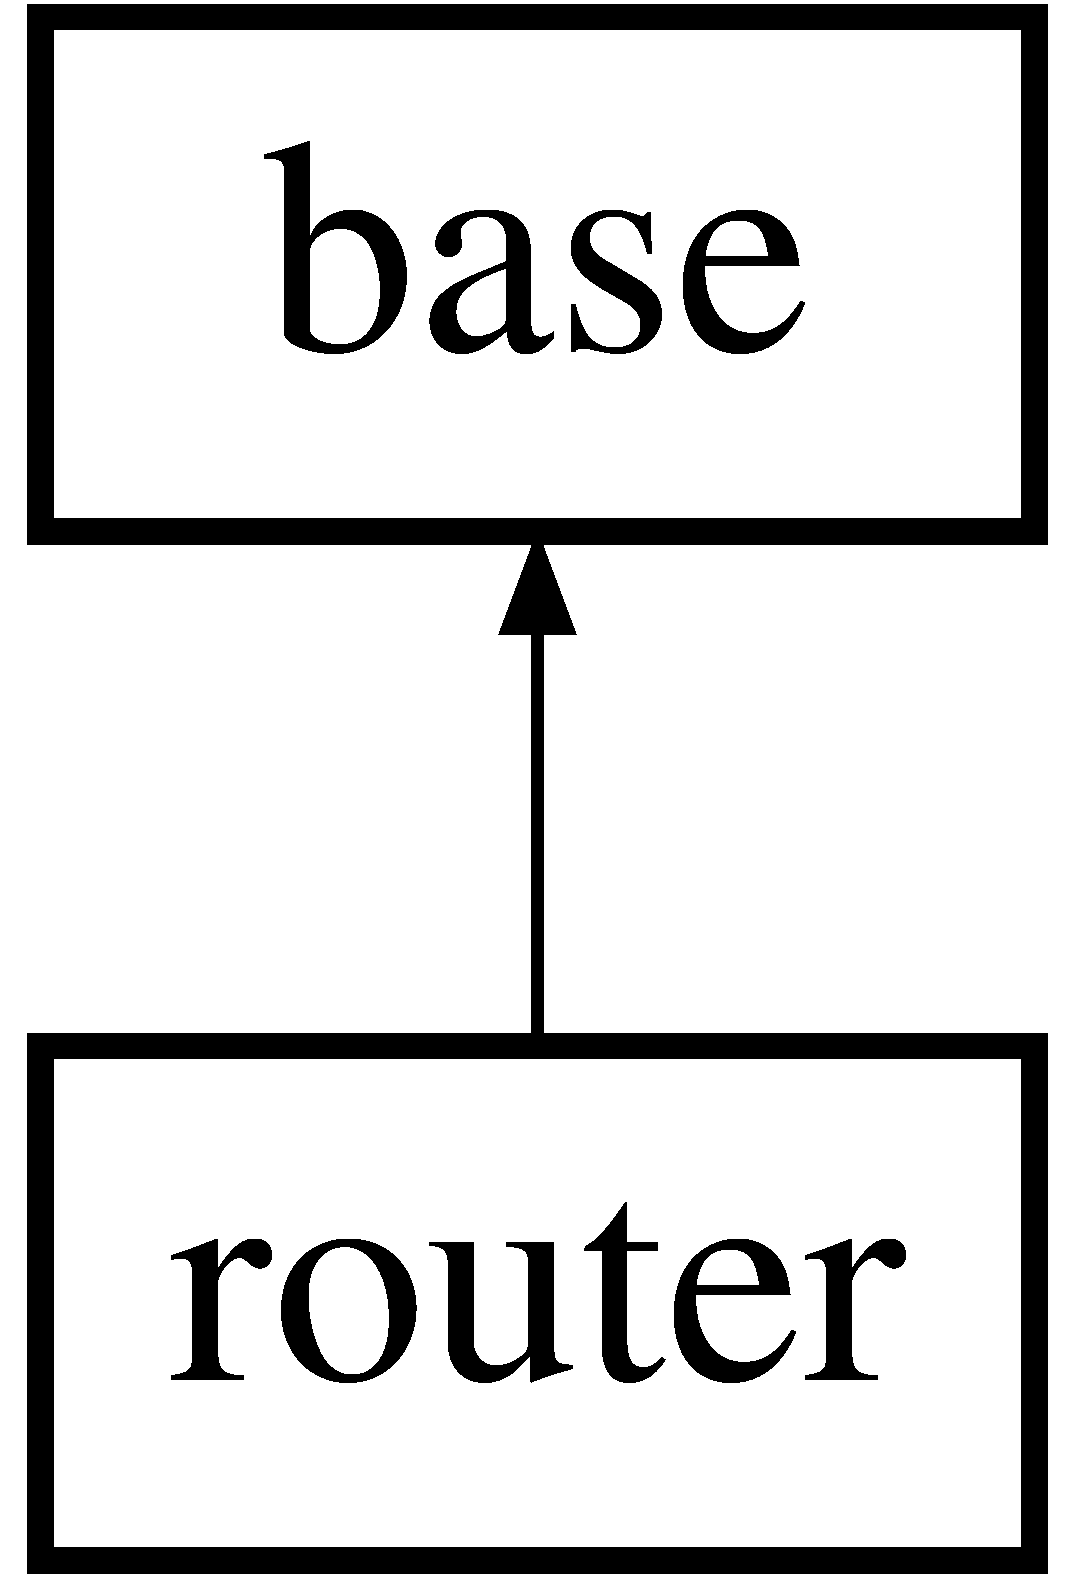
\includegraphics[height=2.000000cm]{classrouter}
\end{center}
\end{figure}
\subsection*{Static Public Member Functions}
\begin{DoxyCompactItemize}
\item 
static \hyperlink{classrouter_aafd29366ef6399da1dd079fc131d8858}{route} (\$pattern, \$funcs, \$http= 'GET', \$name=FALSE)
\item 
static \hyperlink{classrouter_ad3a572002fd350672b531756f7306e8f}{run} ()
\item 
static \hyperlink{classrouter_a2c24b81993e81c6401edd6c4caff0336}{urlFor} (\$name, \$params=array())
\end{DoxyCompactItemize}
\subsection*{Static Private Member Functions}
\begin{DoxyCompactItemize}
\item 
static \hyperlink{classrouter_a78ab5fc58d307458ac8767f50178fc7a}{matches} (\$route)
\end{DoxyCompactItemize}


\subsection{Member Function Documentation}
\hypertarget{classrouter_a78ab5fc58d307458ac8767f50178fc7a}{
\index{router@{router}!matches@{matches}}
\index{matches@{matches}!router@{router}}
\subsubsection[{matches}]{\setlength{\rightskip}{0pt plus 5cm}static matches (
\begin{DoxyParamCaption}
\item[{\$}]{route}
\end{DoxyParamCaption}
)\hspace{0.3cm}{\ttfamily  \mbox{[}static, private\mbox{]}}}}
\label{classrouter_a78ab5fc58d307458ac8767f50178fc7a}
Checks if \$route matches the current URL 
\begin{DoxyParams}[1]{Parameters}
string & {\em \$route} & \\
\hline
\end{DoxyParams}

\begin{DoxyRetVals}{Return values}
{\em true} & \\
\hline
{\em false} & \\
\hline
\end{DoxyRetVals}
\hypertarget{classrouter_aafd29366ef6399da1dd079fc131d8858}{
\index{router@{router}!route@{route}}
\index{route@{route}!router@{router}}
\subsubsection[{route}]{\setlength{\rightskip}{0pt plus 5cm}static route (
\begin{DoxyParamCaption}
\item[{\$}]{pattern, }
\item[{\$}]{funcs, }
\item[{\$}]{http = {\ttfamily 'GET'}, }
\item[{\$}]{name = {\ttfamily FALSE}}
\end{DoxyParamCaption}
)\hspace{0.3cm}{\ttfamily  \mbox{[}static\mbox{]}}}}
\label{classrouter_aafd29366ef6399da1dd079fc131d8858}
Assign handler to route pattern 
\begin{DoxyParams}[1]{Parameters}
string & {\em \$pattern} & \\
\hline
mixed & {\em \$funcs} & \\
\hline
string & {\em \$http} & \\
\hline
string & {\em \$name} & \\
\hline
\end{DoxyParams}
\hypertarget{classrouter_ad3a572002fd350672b531756f7306e8f}{
\index{router@{router}!run@{run}}
\index{run@{run}!router@{router}}
\subsubsection[{run}]{\setlength{\rightskip}{0pt plus 5cm}static run (
\begin{DoxyParamCaption}
{}
\end{DoxyParamCaption}
)\hspace{0.3cm}{\ttfamily  \mbox{[}static\mbox{]}}}}
\label{classrouter_ad3a572002fd350672b531756f7306e8f}
Process routes based on incoming URI. URL that is not matched will be passed as arguments to the functions that are called \hypertarget{classrouter_a2c24b81993e81c6401edd6c4caff0336}{
\index{router@{router}!urlFor@{urlFor}}
\index{urlFor@{urlFor}!router@{router}}
\subsubsection[{urlFor}]{\setlength{\rightskip}{0pt plus 5cm}static urlFor (
\begin{DoxyParamCaption}
\item[{\$}]{name, }
\item[{\$}]{params = {\ttfamily array()}}
\end{DoxyParamCaption}
)\hspace{0.3cm}{\ttfamily  \mbox{[}static\mbox{]}}}}
\label{classrouter_a2c24b81993e81c6401edd6c4caff0336}
Returns a URL with values for a given routing pattern 
\begin{DoxyParams}[1]{Parameters}
string & {\em \$name} & \\
\hline
array & {\em \$params} & \\
\hline
\end{DoxyParams}
\begin{DoxyReturn}{Returns}
string 
\end{DoxyReturn}


The documentation for this class was generated from the following file:\begin{DoxyCompactItemize}
\item 
C:/wamp/www/framework/\hyperlink{router_8php}{router.php}\end{DoxyCompactItemize}

\hypertarget{classtable}{
\section{table Class Reference}
\label{classtable}\index{table@{table}}
}
Inheritance diagram for table:\begin{figure}[H]
\begin{center}
\leavevmode
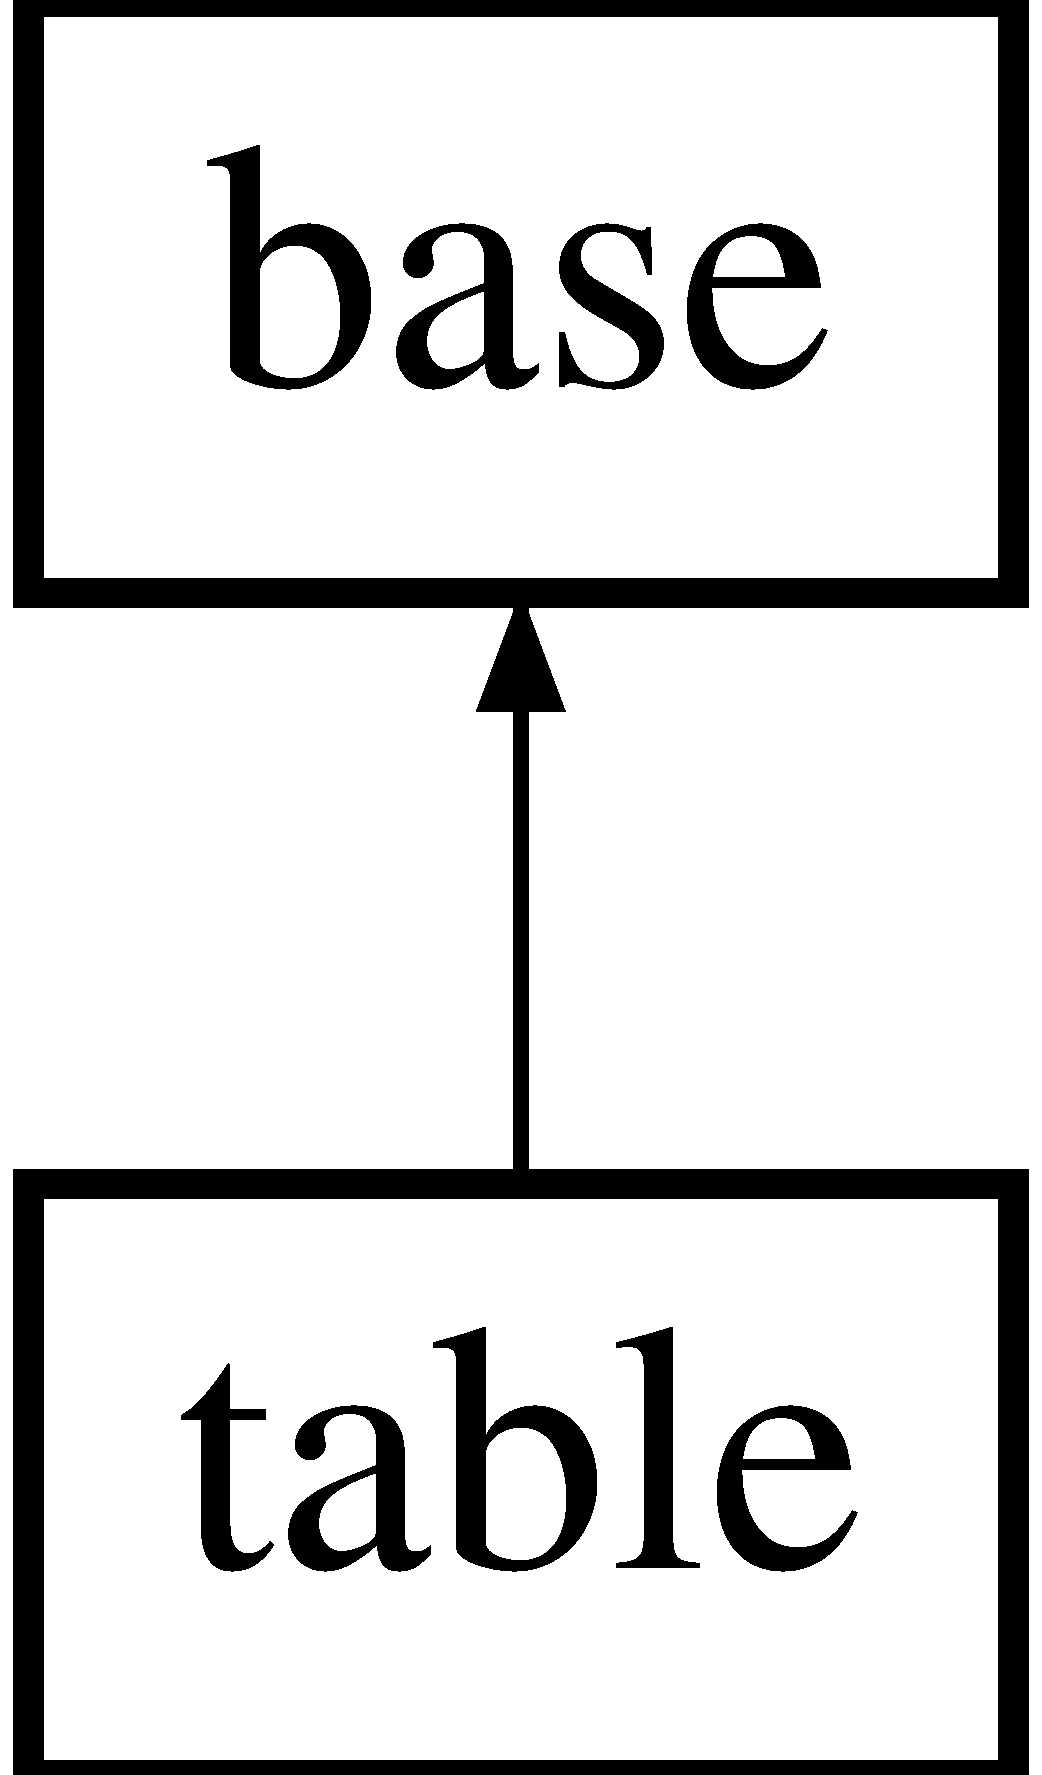
\includegraphics[height=2.000000cm]{classtable}
\end{center}
\end{figure}
\subsection*{Public Member Functions}
\begin{DoxyCompactItemize}
\item 
\hyperlink{classtable_adb8d24f1376e0b2c5f31deb281c76385}{\_\-\_\-construct} (\$\hyperlink{classtable}{table}, \$id=FALSE, \$columns=FALSE, \$connection=FALSE)
\item 
\hyperlink{classtable_a83c2703c91959192f759992ad5640b67}{\_\-\_\-set} (\$name, \$value)
\item 
\hyperlink{classtable_abc8e9e31bb15c8a44c3210ec551407c8}{\_\-\_\-get} (\$name)
\item 
\hyperlink{classtable_a8f132f051b7cd7d570ccb9f6e2bb4201}{\_\-\_\-isset} (\$name)
\item 
\hyperlink{classtable_aaf11785905da71774e052912d784e3b4}{\_\-\_\-sleep} ()
\item 
\hyperlink{classtable_af231e86ad32039b9573ae228db5a29fa}{\_\-\_\-call} (\$name, \$args)
\item 
\hyperlink{classtable_ae671e339cdf6b77d4f8a9f6288000502}{getPrimaryKey} (\$value=FALSE)
\item 
\hyperlink{classtable_ac1eeb13dfaefd70b4c778080e5330525}{getData} (\$object=FALSE)
\item 
\hyperlink{classtable_afc8a3c62679cf00ade9f15fb2a6d6132}{save} ()
\item 
\hyperlink{classtable_a13bdffdd926f26b825ea57066334ff01}{delete} ()
\item 
\hyperlink{classtable_a144f2a49e9970315392c13525d5de652}{find} (\$\hyperlink{classtable}{table}, \$filters=array(), \$ordergroup=array(), \$columns=array())
\item 
\hyperlink{classtable_a456b3964c514406cc9498fc49e8c0317}{countRows} (\$\hyperlink{classtable}{table}, \$filters=array(), \$ordergroup=array())
\item 
\hyperlink{classtable_aa86daa58bc1ff877f2137c27b222dff6}{addRelation} (\$tablename, \$arg1, \$arg2=FALSE)
\item 
\hyperlink{classtable_a29c2012e7cc6b182cc3ca63acfc324b9}{addRelationM2M} (\$connectortable, \$thisid, \$mappedid, \$connectedtable, \$thatid, \$cmappedid)
\item 
\hyperlink{classtable_ac228d1f699104433c0f2679dd2dacdaf}{setAll} (\$values)
\end{DoxyCompactItemize}
\subsection*{Static Public Member Functions}
\begin{DoxyCompactItemize}
\item 
static \hyperlink{classtable_a0b7ba4f111f6cd48fadd4c61966cc308}{importRows} (\$\hyperlink{classtable}{table}, \$values)
\item 
static \hyperlink{classtable_a6c52ede0b29dff2c2aaf5a9f7c220de0}{set} (\$\hyperlink{classtable}{table}, \$id=FALSE, \$columns=FALSE, \$connection=FALSE)
\item 
static \hyperlink{classtable_a9b398e8dfd316739e74a7d19f2d988f0}{addRelationM2MS} (\$\hyperlink{classtable}{table}, \$connectortable, \$thisid, \$mappedid, \$connectedtable, \$thatid, \$cmappedid)
\item 
static \hyperlink{classtable_aa3af4eeabe0a499ae25ef80fc93abbbd}{addRelationS} (\$\hyperlink{classtable}{table}, \$tablename, \$arg1, \$arg2=FALSE)
\item 
static \hyperlink{classtable_ae5daa73e570561db01a6198d85c50a1d}{findS} (\$\hyperlink{classtable}{table}, \$filters=array(), \$ordergroup=array(), \$columns=array())
\end{DoxyCompactItemize}
\subsection*{Data Fields}
\begin{DoxyCompactItemize}
\item 
\hyperlink{classtable_ae8876a14058f368335baccf35af4a22b}{\$table}
\end{DoxyCompactItemize}
\subsection*{Static Public Attributes}
\begin{DoxyCompactItemize}
\item 
static \hyperlink{classtable_a3d332a3c374a53802495dcb045f6133f}{\$tables} = array()
\item 
static \hyperlink{classtable_a5787b67dccb801e89f4ff779d42edece}{\$relations} = array()
\end{DoxyCompactItemize}
\subsection*{Private Member Functions}
\begin{DoxyCompactItemize}
\item 
\hyperlink{classtable_acd2fc9d3975a06de8837cbb9086eebd3}{hydrate} (\$id)
\item 
\hyperlink{classtable_a6287262cb9628d7a89d8fc16dcb51177}{getColumns} ()
\item 
\hyperlink{classtable_a143749a0fde8ad809f2be26ff1f9fcbd}{analyzeRelations} ()
\end{DoxyCompactItemize}
\subsection*{Private Attributes}
\begin{DoxyCompactItemize}
\item 
\hyperlink{classtable_a0d9c79b9b86b3f5891c6d3892f12c6a0}{\$connection}
\item 
\hyperlink{classtable_a2b8d61dccac79ff04332cba49ed5b1cb}{\$originalData} = array()
\item 
\hyperlink{classtable_aa6f12825505c804bc03b634a7598eb45}{\$modifiedData} = array()
\end{DoxyCompactItemize}
\subsection*{Static Private Attributes}
\begin{DoxyCompactItemize}
\item 
static \hyperlink{classtable_a927b0256b942a3ee89485f2649af7981}{\$primaryKey} = array()
\end{DoxyCompactItemize}


\subsection{Detailed Description}
Provides CRUD and ORM functionality. Detects automatically all the columns of a table. 

\subsection{Constructor \& Destructor Documentation}
\hypertarget{classtable_adb8d24f1376e0b2c5f31deb281c76385}{
\index{table@{table}!\_\-\_\-construct@{\_\-\_\-construct}}
\index{\_\-\_\-construct@{\_\-\_\-construct}!table@{table}}
\subsubsection[{\_\-\_\-construct}]{\setlength{\rightskip}{0pt plus 5cm}\_\-\_\-construct (
\begin{DoxyParamCaption}
\item[{\$}]{table, }
\item[{\$}]{id = {\ttfamily FALSE}, }
\item[{\$}]{columns = {\ttfamily FALSE}, }
\item[{\$}]{connection = {\ttfamily FALSE}}
\end{DoxyParamCaption}
)}}
\label{classtable_adb8d24f1376e0b2c5f31deb281c76385}
Initializes the table. 
\begin{DoxyParams}[1]{Parameters}
string & {\em \$table} & \\
\hline
int & {\em \$id} & \\
\hline
array & {\em \$columns} & \\
\hline
\hyperlink{interfacedatabase_adapter}{databaseAdapter} & {\em \$connection} & \\
\hline
\end{DoxyParams}


\subsection{Member Function Documentation}
\hypertarget{classtable_af231e86ad32039b9573ae228db5a29fa}{
\index{table@{table}!\_\-\_\-call@{\_\-\_\-call}}
\index{\_\-\_\-call@{\_\-\_\-call}!table@{table}}
\subsubsection[{\_\-\_\-call}]{\setlength{\rightskip}{0pt plus 5cm}\_\-\_\-call (
\begin{DoxyParamCaption}
\item[{\$}]{name, }
\item[{\$}]{args}
\end{DoxyParamCaption}
)}}
\label{classtable_af231e86ad32039b9573ae228db5a29fa}
Magic method for setting or getting related tables. If function is called without argument, it will find the related tables. If function is called with a related table as an argument, it will be connected to it. 
\begin{DoxyParams}[1]{Parameters}
string & {\em \$name} & \\
\hline
array & {\em \$args} & \\
\hline
\end{DoxyParams}
\begin{Desc}
\item[\hyperlink{todo__todo000006}{Todo}]\$args could be a table of \$name \end{Desc}
\hypertarget{classtable_abc8e9e31bb15c8a44c3210ec551407c8}{
\index{table@{table}!\_\-\_\-get@{\_\-\_\-get}}
\index{\_\-\_\-get@{\_\-\_\-get}!table@{table}}
\subsubsection[{\_\-\_\-get}]{\setlength{\rightskip}{0pt plus 5cm}\_\-\_\-get (
\begin{DoxyParamCaption}
\item[{\$}]{name}
\end{DoxyParamCaption}
)}}
\label{classtable_abc8e9e31bb15c8a44c3210ec551407c8}
Magic method for accesing dynamic properties 
\begin{DoxyParams}[1]{Parameters}
string & {\em \$name} & \\
\hline
\end{DoxyParams}
\begin{DoxyReturn}{Returns}
mixed 
\end{DoxyReturn}
\hypertarget{classtable_a8f132f051b7cd7d570ccb9f6e2bb4201}{
\index{table@{table}!\_\-\_\-isset@{\_\-\_\-isset}}
\index{\_\-\_\-isset@{\_\-\_\-isset}!table@{table}}
\subsubsection[{\_\-\_\-isset}]{\setlength{\rightskip}{0pt plus 5cm}\_\-\_\-isset (
\begin{DoxyParamCaption}
\item[{\$}]{name}
\end{DoxyParamCaption}
)}}
\label{classtable_a8f132f051b7cd7d570ccb9f6e2bb4201}
Magic method that checks if a column exists 
\begin{DoxyParams}[1]{Parameters}
string & {\em \$name} & \\
\hline
\end{DoxyParams}

\begin{DoxyRetVals}{Return values}
{\em true} & \\
\hline
{\em false} & \\
\hline
\end{DoxyRetVals}
\hypertarget{classtable_a83c2703c91959192f759992ad5640b67}{
\index{table@{table}!\_\-\_\-set@{\_\-\_\-set}}
\index{\_\-\_\-set@{\_\-\_\-set}!table@{table}}
\subsubsection[{\_\-\_\-set}]{\setlength{\rightskip}{0pt plus 5cm}\_\-\_\-set (
\begin{DoxyParamCaption}
\item[{\$}]{name, }
\item[{\$}]{value}
\end{DoxyParamCaption}
)}}
\label{classtable_a83c2703c91959192f759992ad5640b67}
Magic method for setting dynamic properties 
\begin{DoxyParams}[1]{Parameters}
string & {\em \$name} & \\
\hline
string & {\em \$value} & \\
\hline
\end{DoxyParams}
\hypertarget{classtable_aaf11785905da71774e052912d784e3b4}{
\index{table@{table}!\_\-\_\-sleep@{\_\-\_\-sleep}}
\index{\_\-\_\-sleep@{\_\-\_\-sleep}!table@{table}}
\subsubsection[{\_\-\_\-sleep}]{\setlength{\rightskip}{0pt plus 5cm}\_\-\_\-sleep (
\begin{DoxyParamCaption}
{}
\end{DoxyParamCaption}
)}}
\label{classtable_aaf11785905da71774e052912d784e3b4}
Magic method for serialization \hypertarget{classtable_aa86daa58bc1ff877f2137c27b222dff6}{
\index{table@{table}!addRelation@{addRelation}}
\index{addRelation@{addRelation}!table@{table}}
\subsubsection[{addRelation}]{\setlength{\rightskip}{0pt plus 5cm}addRelation (
\begin{DoxyParamCaption}
\item[{\$}]{tablename, }
\item[{\$}]{arg1, }
\item[{\$}]{arg2 = {\ttfamily FALSE}}
\end{DoxyParamCaption}
)}}
\label{classtable_aa86daa58bc1ff877f2137c27b222dff6}
Adds a relation to another table. This is not for many to many tables. Use addRelationM2M for that. If third argument isn't passed, it defaults to the table primary key. Returns the table we are working on, to allow chaining of methods. 
\begin{DoxyParams}[1]{Parameters}
string & {\em \$tablename} & \\
\hline
string & {\em \$arg1} & \\
\hline
string & {\em \$arg2} & \\
\hline
\end{DoxyParams}
\begin{DoxyReturn}{Returns}
\$this 
\end{DoxyReturn}
\hypertarget{classtable_a29c2012e7cc6b182cc3ca63acfc324b9}{
\index{table@{table}!addRelationM2M@{addRelationM2M}}
\index{addRelationM2M@{addRelationM2M}!table@{table}}
\subsubsection[{addRelationM2M}]{\setlength{\rightskip}{0pt plus 5cm}addRelationM2M (
\begin{DoxyParamCaption}
\item[{\$}]{connectortable, }
\item[{\$}]{thisid, }
\item[{\$}]{mappedid, }
\item[{\$}]{connectedtable, }
\item[{\$}]{thatid, }
\item[{\$}]{cmappedid}
\end{DoxyParamCaption}
)}}
\label{classtable_a29c2012e7cc6b182cc3ca63acfc324b9}
Adds a many-\/to-\/many relation between tables. Takes a crapload of arguments. Returns the table we are working on, to allow chaining of methods. 
\begin{DoxyParams}[1]{Parameters}
string & {\em \$connectortable} & \\
\hline
string & {\em \$thisid} & \\
\hline
string & {\em \$mappedid} & \\
\hline
string & {\em \$connectedtable} & \\
\hline
string & {\em \$thatid} & \\
\hline
string & {\em \$cmappedid} & \\
\hline
\end{DoxyParams}
\begin{Desc}
\item[\hyperlink{todo__todo000007}{Todo}]find a way to reduce arguments \end{Desc}
\begin{DoxyReturn}{Returns}
\$this 
\end{DoxyReturn}
\hypertarget{classtable_a9b398e8dfd316739e74a7d19f2d988f0}{
\index{table@{table}!addRelationM2MS@{addRelationM2MS}}
\index{addRelationM2MS@{addRelationM2MS}!table@{table}}
\subsubsection[{addRelationM2MS}]{\setlength{\rightskip}{0pt plus 5cm}static addRelationM2MS (
\begin{DoxyParamCaption}
\item[{\$}]{table, }
\item[{\$}]{connectortable, }
\item[{\$}]{thisid, }
\item[{\$}]{mappedid, }
\item[{\$}]{connectedtable, }
\item[{\$}]{thatid, }
\item[{\$}]{cmappedid}
\end{DoxyParamCaption}
)\hspace{0.3cm}{\ttfamily  \mbox{[}static\mbox{]}}}}
\label{classtable_a9b398e8dfd316739e74a7d19f2d988f0}
Adds a Many-\/To-\/Many relationship statically. See \hyperlink{classtable_a29c2012e7cc6b182cc3ca63acfc324b9}{addRelationM2M()}. 
\begin{DoxyParams}[1]{Parameters}
string & {\em \$table} & The table from which to start the relation \\
\hline
string & {\em \$connectortable} & \\
\hline
string & {\em \$thisid} & \\
\hline
string & {\em \$mappedid} & \\
\hline
string & {\em \$connectedtable} & \\
\hline
string & {\em \$thatid} & \\
\hline
string & {\em \$cmappedid} & \\
\hline
\end{DoxyParams}
\hypertarget{classtable_aa3af4eeabe0a499ae25ef80fc93abbbd}{
\index{table@{table}!addRelationS@{addRelationS}}
\index{addRelationS@{addRelationS}!table@{table}}
\subsubsection[{addRelationS}]{\setlength{\rightskip}{0pt plus 5cm}static addRelationS (
\begin{DoxyParamCaption}
\item[{\$}]{table, }
\item[{\$}]{tablename, }
\item[{\$}]{arg1, }
\item[{\$}]{arg2 = {\ttfamily FALSE}}
\end{DoxyParamCaption}
)\hspace{0.3cm}{\ttfamily  \mbox{[}static\mbox{]}}}}
\label{classtable_aa3af4eeabe0a499ae25ef80fc93abbbd}
Adds a relation to another table statically. See \hyperlink{classtable_aa86daa58bc1ff877f2137c27b222dff6}{addRelation()}. 
\begin{DoxyParams}[1]{Parameters}
string & {\em \$table} & The table from which to start the relation \\
\hline
string & {\em \$tablename} & \\
\hline
string & {\em \$arg1} & \\
\hline
string & {\em \$arg2} & \\
\hline
\end{DoxyParams}
\hypertarget{classtable_a143749a0fde8ad809f2be26ff1f9fcbd}{
\index{table@{table}!analyzeRelations@{analyzeRelations}}
\index{analyzeRelations@{analyzeRelations}!table@{table}}
\subsubsection[{analyzeRelations}]{\setlength{\rightskip}{0pt plus 5cm}analyzeRelations (
\begin{DoxyParamCaption}
{}
\end{DoxyParamCaption}
)\hspace{0.3cm}{\ttfamily  \mbox{[}private\mbox{]}}}}
\label{classtable_a143749a0fde8ad809f2be26ff1f9fcbd}
Analyzes the relation between tables and marks them accordingly. So far only ONE TO MANY and MANY TO MANY ones. Haven't seen a case of single \hypertarget{classtable_a456b3964c514406cc9498fc49e8c0317}{
\index{table@{table}!countRows@{countRows}}
\index{countRows@{countRows}!table@{table}}
\subsubsection[{countRows}]{\setlength{\rightskip}{0pt plus 5cm}countRows (
\begin{DoxyParamCaption}
\item[{\$}]{table, }
\item[{\$}]{filters = {\ttfamily array()}, }
\item[{\$}]{ordergroup = {\ttfamily array()}}
\end{DoxyParamCaption}
)}}
\label{classtable_a456b3964c514406cc9498fc49e8c0317}
Returns the number of rows that result from a SELECT query. Parameters are the same as for \hyperlink{classtable_a144f2a49e9970315392c13525d5de652}{find()}, except that you can't return only some columns. Also, ordering is not included in the query. 
\begin{DoxyParams}[1]{Parameters}
string & {\em \$table} & Table in which to search \\
\hline
array & {\em \$filters} & Filters to apply. Can be name=$>$value pair, SQL statement, or recursive array relating to conditions on other tables \\
\hline
array & {\em \$ordergroup} & How to order, group and limit the search \\
\hline
\end{DoxyParams}
\begin{DoxyReturn}{Returns}
int 
\end{DoxyReturn}
\hypertarget{classtable_a13bdffdd926f26b825ea57066334ff01}{
\index{table@{table}!delete@{delete}}
\index{delete@{delete}!table@{table}}
\subsubsection[{delete}]{\setlength{\rightskip}{0pt plus 5cm}delete (
\begin{DoxyParamCaption}
{}
\end{DoxyParamCaption}
)}}
\label{classtable_a13bdffdd926f26b825ea57066334ff01}
Delete the corresponding record from the database \hypertarget{classtable_a144f2a49e9970315392c13525d5de652}{
\index{table@{table}!find@{find}}
\index{find@{find}!table@{table}}
\subsubsection[{find}]{\setlength{\rightskip}{0pt plus 5cm}find (
\begin{DoxyParamCaption}
\item[{\$}]{table, }
\item[{\$}]{filters = {\ttfamily array()}, }
\item[{\$}]{ordergroup = {\ttfamily array()}, }
\item[{\$}]{columns = {\ttfamily array()}}
\end{DoxyParamCaption}
)}}
\label{classtable_a144f2a49e9970315392c13525d5de652}
Makes and executes a SQL query, based on various filters, orders, groups, and columns to return. 
\begin{DoxyParams}[1]{Parameters}
string & {\em \$table} & Table in which to search \\
\hline
array & {\em \$filters} & Filters to apply. Can be name=$>$value pair, SQL statement, or recursive array relating to conditions on other tables \\
\hline
array & {\em \$ordergroup} & How to order, group and limit the search \\
\hline
array & {\em \$columns} & What columns to return in search \\
\hline
\end{DoxyParams}
\begin{DoxyReturn}{Returns}
array 
\end{DoxyReturn}
\hypertarget{classtable_ae5daa73e570561db01a6198d85c50a1d}{
\index{table@{table}!findS@{findS}}
\index{findS@{findS}!table@{table}}
\subsubsection[{findS}]{\setlength{\rightskip}{0pt plus 5cm}static findS (
\begin{DoxyParamCaption}
\item[{\$}]{table, }
\item[{\$}]{filters = {\ttfamily array()}, }
\item[{\$}]{ordergroup = {\ttfamily array()}, }
\item[{\$}]{columns = {\ttfamily array()}}
\end{DoxyParamCaption}
)\hspace{0.3cm}{\ttfamily  \mbox{[}static\mbox{]}}}}
\label{classtable_ae5daa73e570561db01a6198d85c50a1d}
Static wrapper for \hyperlink{classtable_a144f2a49e9970315392c13525d5de652}{find()}. Arguments the same. 
\begin{DoxyParams}[1]{Parameters}
string & {\em \$table} & Table in which to search \\
\hline
array & {\em \$filters} & Filters to apply. Can be name=$>$value pair, SQL statement, or recursive array relating to conditions on other tables \\
\hline
array & {\em \$ordergroup} & How to order, group and limit the search \\
\hline
array & {\em \$columns} & What columns to return in search \\
\hline
\end{DoxyParams}
\begin{DoxyReturn}{Returns}
array 
\end{DoxyReturn}
\hypertarget{classtable_a6287262cb9628d7a89d8fc16dcb51177}{
\index{table@{table}!getColumns@{getColumns}}
\index{getColumns@{getColumns}!table@{table}}
\subsubsection[{getColumns}]{\setlength{\rightskip}{0pt plus 5cm}getColumns (
\begin{DoxyParamCaption}
{}
\end{DoxyParamCaption}
)\hspace{0.3cm}{\ttfamily  \mbox{[}private\mbox{]}}}}
\label{classtable_a6287262cb9628d7a89d8fc16dcb51177}
Populates the \$data property of the object with the columns of the table and gets the primary key of the table, if it exists \hypertarget{classtable_ac1eeb13dfaefd70b4c778080e5330525}{
\index{table@{table}!getData@{getData}}
\index{getData@{getData}!table@{table}}
\subsubsection[{getData}]{\setlength{\rightskip}{0pt plus 5cm}getData (
\begin{DoxyParamCaption}
\item[{\$}]{object = {\ttfamily FALSE}}
\end{DoxyParamCaption}
)}}
\label{classtable_ac1eeb13dfaefd70b4c778080e5330525}
Returns the values of the current row as a key=$>$value array. If the \$object parameter is set to true, it returns an object with it's properties having the role of key-\/value pairs. If it hasn't been hydrated, it returns false. 
\begin{DoxyParams}[1]{Parameters}
boolena & {\em \$object} & \\
\hline
\end{DoxyParams}
\begin{DoxyReturn}{Returns}
mixed 
\end{DoxyReturn}
\hypertarget{classtable_ae671e339cdf6b77d4f8a9f6288000502}{
\index{table@{table}!getPrimaryKey@{getPrimaryKey}}
\index{getPrimaryKey@{getPrimaryKey}!table@{table}}
\subsubsection[{getPrimaryKey}]{\setlength{\rightskip}{0pt plus 5cm}getPrimaryKey (
\begin{DoxyParamCaption}
\item[{\$}]{value = {\ttfamily FALSE}}
\end{DoxyParamCaption}
)}}
\label{classtable_ae671e339cdf6b77d4f8a9f6288000502}
Returns the primary key of this table. If \$value is TRUE, then it returns the value of the primary key for this row 
\begin{DoxyParams}[1]{Parameters}
bool & {\em \$value} & \\
\hline
\end{DoxyParams}

\begin{DoxyRetVals}{Return values}
{\em int} & Value of the primary key \\
\hline
{\em string} & The name of the primary key \\
\hline
\end{DoxyRetVals}
\hypertarget{classtable_acd2fc9d3975a06de8837cbb9086eebd3}{
\index{table@{table}!hydrate@{hydrate}}
\index{hydrate@{hydrate}!table@{table}}
\subsubsection[{hydrate}]{\setlength{\rightskip}{0pt plus 5cm}hydrate (
\begin{DoxyParamCaption}
\item[{\$}]{id}
\end{DoxyParamCaption}
)\hspace{0.3cm}{\ttfamily  \mbox{[}private\mbox{]}}}}
\label{classtable_acd2fc9d3975a06de8837cbb9086eebd3}
Populate the object with data from the table, selected according to primary key value 
\begin{DoxyParams}[1]{Parameters}
number & {\em \$id} & \\
\hline
\end{DoxyParams}
\begin{DoxyReturn}{Returns}
array 
\end{DoxyReturn}
\hypertarget{classtable_a0b7ba4f111f6cd48fadd4c61966cc308}{
\index{table@{table}!importRows@{importRows}}
\index{importRows@{importRows}!table@{table}}
\subsubsection[{importRows}]{\setlength{\rightskip}{0pt plus 5cm}static importRows (
\begin{DoxyParamCaption}
\item[{\$}]{table, }
\item[{\$}]{values}
\end{DoxyParamCaption}
)\hspace{0.3cm}{\ttfamily  \mbox{[}static\mbox{]}}}}
\label{classtable_a0b7ba4f111f6cd48fadd4c61966cc308}
Imports an array of rows and returns an array of table objects filled with values. If there is only one row in \$values, it returns it as an object instead of as an array. 
\begin{DoxyParams}[1]{Parameters}
string & {\em \$table} & \\
\hline
array & {\em \$values} & \\
\hline
\end{DoxyParams}
\begin{DoxyReturn}{Returns}
array 
\end{DoxyReturn}
\hypertarget{classtable_afc8a3c62679cf00ade9f15fb2a6d6132}{
\index{table@{table}!save@{save}}
\index{save@{save}!table@{table}}
\subsubsection[{save}]{\setlength{\rightskip}{0pt plus 5cm}save (
\begin{DoxyParamCaption}
{}
\end{DoxyParamCaption}
)}}
\label{classtable_afc8a3c62679cf00ade9f15fb2a6d6132}
Save changes made to object. If the object was hydrated, it will be updated. If it was created from scratch, it will be inserted into the database 
\begin{DoxyRetVals}{Return values}
{\em true} & If modifying was succesfull \\
\hline
{\em int} & If a row was inserted, it returns the insert ID \\
\hline
{\em false} & If there was an error \\
\hline
\end{DoxyRetVals}
\hypertarget{classtable_a6c52ede0b29dff2c2aaf5a9f7c220de0}{
\index{table@{table}!set@{set}}
\index{set@{set}!table@{table}}
\subsubsection[{set}]{\setlength{\rightskip}{0pt plus 5cm}static set (
\begin{DoxyParamCaption}
\item[{\$}]{table, }
\item[{\$}]{id = {\ttfamily FALSE}, }
\item[{\$}]{columns = {\ttfamily FALSE}, }
\item[{\$}]{connection = {\ttfamily FALSE}}
\end{DoxyParamCaption}
)\hspace{0.3cm}{\ttfamily  \mbox{[}static\mbox{]}}}}
\label{classtable_a6c52ede0b29dff2c2aaf5a9f7c220de0}
Static convenience wrapper functions Initializes a certain table 
\begin{DoxyParams}[1]{Parameters}
string & {\em \$table} & \\
\hline
int & {\em \$id} & \\
\hline
array & {\em \$columns} & \\
\hline
\hyperlink{interfacedatabase_adapter}{databaseAdapter} & {\em \$connection} & \\
\hline
\end{DoxyParams}
\hypertarget{classtable_ac228d1f699104433c0f2679dd2dacdaf}{
\index{table@{table}!setAll@{setAll}}
\index{setAll@{setAll}!table@{table}}
\subsubsection[{setAll}]{\setlength{\rightskip}{0pt plus 5cm}setAll (
\begin{DoxyParamCaption}
\item[{\$}]{values}
\end{DoxyParamCaption}
)}}
\label{classtable_ac228d1f699104433c0f2679dd2dacdaf}
Set all the values of row at once. It doesn't save the row to the database. 
\begin{DoxyParams}[1]{Parameters}
array & {\em \$values} & \\
\hline
\end{DoxyParams}


\subsection{Field Documentation}
\hypertarget{classtable_a0d9c79b9b86b3f5891c6d3892f12c6a0}{
\index{table@{table}!\$connection@{\$connection}}
\index{\$connection@{\$connection}!table@{table}}
\subsubsection[{\$connection}]{\setlength{\rightskip}{0pt plus 5cm}\$connection\hspace{0.3cm}{\ttfamily  \mbox{[}private\mbox{]}}}}
\label{classtable_a0d9c79b9b86b3f5891c6d3892f12c6a0}
\hypertarget{classtable_aa6f12825505c804bc03b634a7598eb45}{
\index{table@{table}!\$modifiedData@{\$modifiedData}}
\index{\$modifiedData@{\$modifiedData}!table@{table}}
\subsubsection[{\$modifiedData}]{\setlength{\rightskip}{0pt plus 5cm}\$modifiedData = array()\hspace{0.3cm}{\ttfamily  \mbox{[}private\mbox{]}}}}
\label{classtable_aa6f12825505c804bc03b634a7598eb45}
\hypertarget{classtable_a2b8d61dccac79ff04332cba49ed5b1cb}{
\index{table@{table}!\$originalData@{\$originalData}}
\index{\$originalData@{\$originalData}!table@{table}}
\subsubsection[{\$originalData}]{\setlength{\rightskip}{0pt plus 5cm}\$originalData = array()\hspace{0.3cm}{\ttfamily  \mbox{[}private\mbox{]}}}}
\label{classtable_a2b8d61dccac79ff04332cba49ed5b1cb}
\hypertarget{classtable_a927b0256b942a3ee89485f2649af7981}{
\index{table@{table}!\$primaryKey@{\$primaryKey}}
\index{\$primaryKey@{\$primaryKey}!table@{table}}
\subsubsection[{\$primaryKey}]{\setlength{\rightskip}{0pt plus 5cm}\$primaryKey = array()\hspace{0.3cm}{\ttfamily  \mbox{[}static, private\mbox{]}}}}
\label{classtable_a927b0256b942a3ee89485f2649af7981}
\hypertarget{classtable_a5787b67dccb801e89f4ff779d42edece}{
\index{table@{table}!\$relations@{\$relations}}
\index{\$relations@{\$relations}!table@{table}}
\subsubsection[{\$relations}]{\setlength{\rightskip}{0pt plus 5cm}\$relations = array()\hspace{0.3cm}{\ttfamily  \mbox{[}static\mbox{]}}}}
\label{classtable_a5787b67dccb801e89f4ff779d42edece}
Static variable containing the relations between tables \hypertarget{classtable_ae8876a14058f368335baccf35af4a22b}{
\index{table@{table}!\$table@{\$table}}
\index{\$table@{\$table}!table@{table}}
\subsubsection[{\$table}]{\setlength{\rightskip}{0pt plus 5cm}\${\bf table}}}
\label{classtable_ae8876a14058f368335baccf35af4a22b}
Contains the table name of this object \hypertarget{classtable_a3d332a3c374a53802495dcb045f6133f}{
\index{table@{table}!\$tables@{\$tables}}
\index{\$tables@{\$tables}!table@{table}}
\subsubsection[{\$tables}]{\setlength{\rightskip}{0pt plus 5cm}\$tables = array()\hspace{0.3cm}{\ttfamily  \mbox{[}static\mbox{]}}}}
\label{classtable_a3d332a3c374a53802495dcb045f6133f}
Static variable containing the columns of all tables that have been instantiated \begin{Desc}
\item[\hyperlink{todo__todo000005}{Todo}]allow objects representing same table, but different columns \end{Desc}


The documentation for this class was generated from the following file:\begin{DoxyCompactItemize}
\item 
C:/wamp/www/framework/\hyperlink{db_8php}{db.php}\end{DoxyCompactItemize}

\section{template Class Reference}
\label{classtemplate}\index{template@{template}}
Inheritance diagram for template:\begin{figure}[H]
\begin{center}
\leavevmode
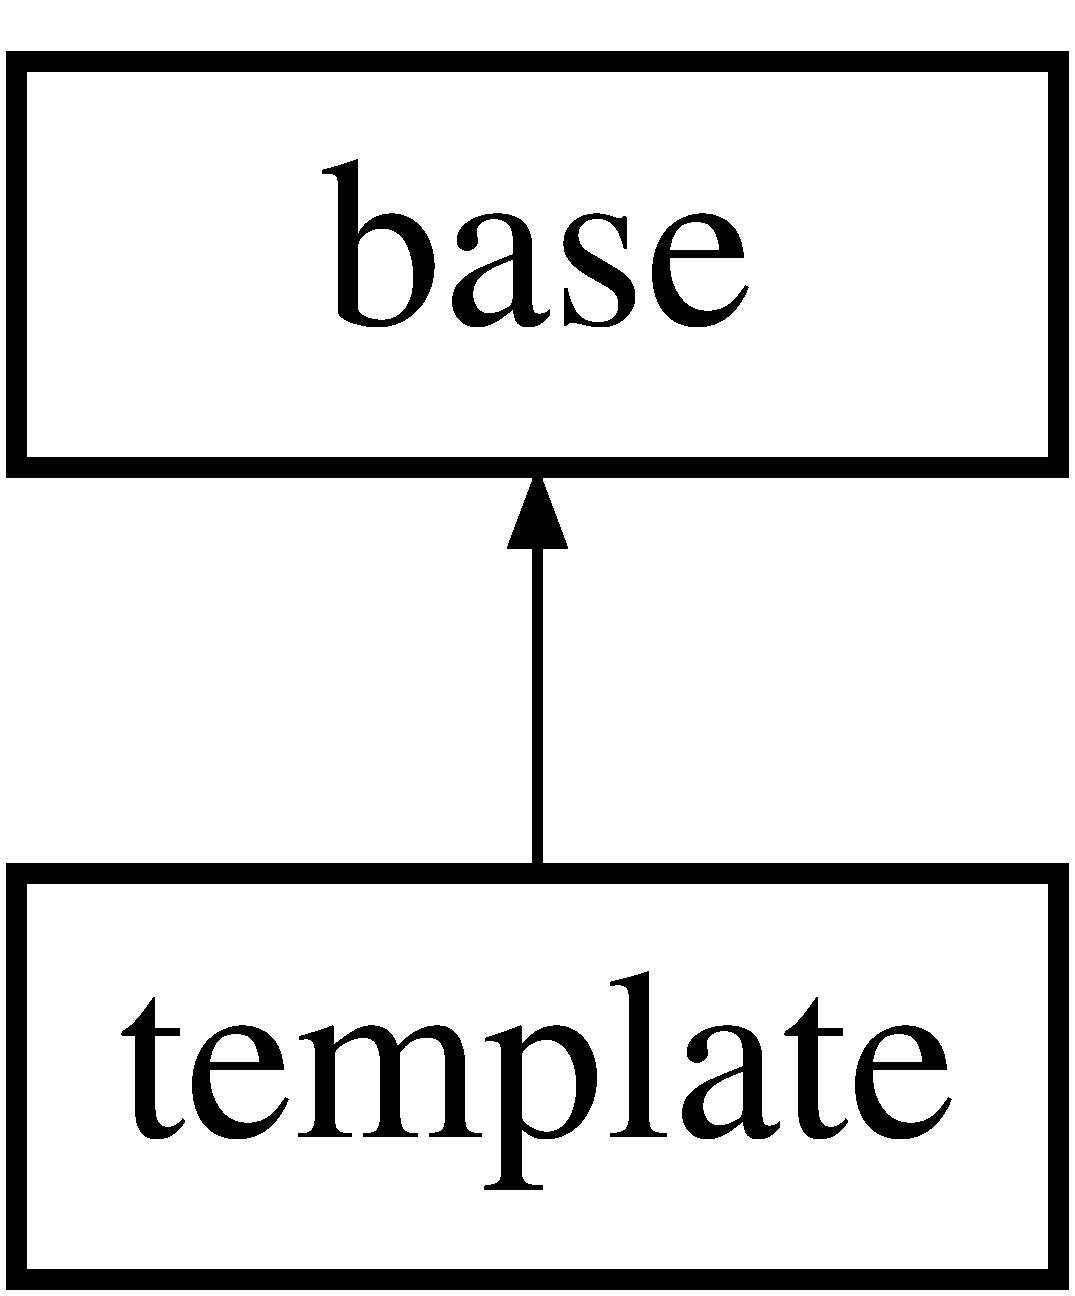
\includegraphics[height=2.000000cm]{classtemplate}
\end{center}
\end{figure}
\subsection*{Public Member Functions}
\begin{DoxyCompactItemize}
\item 
{\bf \_\-\_\-construct} ()
\item 
{\bf \_\-\_\-set} (\$var, \$value=FALSE)
\item 
{\bf assign} (\$var, \$value=FALSE)
\item 
{\bf \_\-\_\-get} (\$name)
\item 
{\bf \_\-\_\-toString} ()
\item 
{\bf view} (\$tpl)
\item 
{\bf getOutput} (\${\bf template})
\item 
{\bf includeSub} (\${\bf template})
\end{DoxyCompactItemize}
\subsection*{Private Member Functions}
\begin{DoxyCompactItemize}
\item 
{\bf checkCompile} (\${\bf template})
\item 
{\bf compile} (\${\bf template})
\end{DoxyCompactItemize}
\subsection*{Static Private Attributes}
\begin{DoxyCompactItemize}
\item 
static {\bf \$values}
\end{DoxyCompactItemize}


\subsection{Detailed Description}
Provides basic templating capabilites 

\subsection{Constructor \& Destructor Documentation}
\index{template@{template}!\_\-\_\-construct@{\_\-\_\-construct}}
\index{\_\-\_\-construct@{\_\-\_\-construct}!template@{template}}
\subsubsection[{\_\-\_\-construct}]{\setlength{\rightskip}{0pt plus 5cm}\_\-\_\-construct (
\begin{DoxyParamCaption}
{}
\end{DoxyParamCaption}
)}\label{classtemplate_a095c5d389db211932136b53f25f39685}
Empty constructor. It's created separately to prevent inheriting the singleton pattern from base. 

Reimplemented from {\bf base} \doxyref{}{p.}{classbase_a095c5d389db211932136b53f25f39685}.



\subsection{Member Function Documentation}
\index{template@{template}!\_\-\_\-get@{\_\-\_\-get}}
\index{\_\-\_\-get@{\_\-\_\-get}!template@{template}}
\subsubsection[{\_\-\_\-get}]{\setlength{\rightskip}{0pt plus 5cm}\_\-\_\-get (
\begin{DoxyParamCaption}
\item[{\$}]{name}
\end{DoxyParamCaption}
)}\label{classtemplate_abc8e9e31bb15c8a44c3210ec551407c8}
Return value of template variable, false if not found. This is separate from the rolisz global variables. 
\begin{DoxyParams}[1]{Parameters}
string & {\em \$name} & \\
\hline
\end{DoxyParams}

\begin{DoxyRetVals}{Return values}
{\em true} & \\
\hline
{\em false} & \\
\hline
\end{DoxyRetVals}
\index{template@{template}!\_\-\_\-set@{\_\-\_\-set}}
\index{\_\-\_\-set@{\_\-\_\-set}!template@{template}}
\subsubsection[{\_\-\_\-set}]{\setlength{\rightskip}{0pt plus 5cm}\_\-\_\-set (
\begin{DoxyParamCaption}
\item[{\$}]{var, }
\item[{\$}]{value = {\ttfamily FALSE}}
\end{DoxyParamCaption}
)}\label{classtemplate_a8ba8e88dc2035039ed49e5d7a9c43093}
Set the value of a template variable magically. If \$var param is string, then a variable called \$var will have the value of \$value. If \$var is array, it should be a key-\/pair value like this array('var\_\-name'=$>$'132','2ndvar'=$>$123). This is separate from the rolisz global variables. 
\begin{DoxyParams}[1]{Parameters}
string | array & {\em \$var} & \\
\hline
mixed & {\em \$value} & \\
\hline
\end{DoxyParams}
\index{template@{template}!\_\-\_\-toString@{\_\-\_\-toString}}
\index{\_\-\_\-toString@{\_\-\_\-toString}!template@{template}}
\subsubsection[{\_\-\_\-toString}]{\setlength{\rightskip}{0pt plus 5cm}\_\-\_\-toString (
\begin{DoxyParamCaption}
{}
\end{DoxyParamCaption}
)}\label{classtemplate_a7516ca30af0db3cdbf9a7739b48ce91d}
Magic method for the serialization of the template object. \begin{DoxyReturn}{Returns}
string containing the template 
\end{DoxyReturn}
\index{template@{template}!assign@{assign}}
\index{assign@{assign}!template@{template}}
\subsubsection[{assign}]{\setlength{\rightskip}{0pt plus 5cm}assign (
\begin{DoxyParamCaption}
\item[{\$}]{var, }
\item[{\$}]{value = {\ttfamily FALSE}}
\end{DoxyParamCaption}
)}\label{classtemplate_aad89b99f86fc0d4fd6a0d0f3f7a15867}
Set the value of a template variable. If \$var param is string, then a variable called \$var will have the value of \$value. If \$var is array, it should be a key-\/pair value like this array('var\_\-name'=$>$'132','2ndvar'=$>$123). This is separate from the rolisz global variables. 
\begin{DoxyParams}[1]{Parameters}
string | array & {\em \$var} & \\
\hline
mixed & {\em \$value} & \\
\hline
\end{DoxyParams}
\index{template@{template}!checkCompile@{checkCompile}}
\index{checkCompile@{checkCompile}!template@{template}}
\subsubsection[{checkCompile}]{\setlength{\rightskip}{0pt plus 5cm}checkCompile (
\begin{DoxyParamCaption}
\item[{\$}]{template}
\end{DoxyParamCaption}
)\hspace{0.3cm}{\ttfamily  [private]}}\label{classtemplate_a57fe1e92cfb84c13658d12becd326984}
Checks if the file has been compiled to the temp folder and if it is more recent than the last change to the template 
\begin{DoxyParams}[1]{Parameters}
string & {\em \$template} & \\
\hline
\end{DoxyParams}

\begin{DoxyRetVals}{Return values}
{\em true} & \\
\hline
{\em false} & \\
\hline
\end{DoxyRetVals}
\index{template@{template}!compile@{compile}}
\index{compile@{compile}!template@{template}}
\subsubsection[{compile}]{\setlength{\rightskip}{0pt plus 5cm}compile (
\begin{DoxyParamCaption}
\item[{\$}]{template}
\end{DoxyParamCaption}
)\hspace{0.3cm}{\ttfamily  [private]}}\label{classtemplate_ab0a641d23ff3291dc8a94085f06b5dee}
Performs the replacing of the shorthand tags to full PHP tags in the \$template file. Places the results in a temp folder, in a file called the md5 value of \$template, to prevent collisions. 
\begin{DoxyParams}[1]{Parameters}
string & {\em \$template} & \\
\hline
\end{DoxyParams}
\index{template@{template}!getOutput@{getOutput}}
\index{getOutput@{getOutput}!template@{template}}
\subsubsection[{getOutput}]{\setlength{\rightskip}{0pt plus 5cm}getOutput (
\begin{DoxyParamCaption}
\item[{\$}]{template}
\end{DoxyParamCaption}
)}\label{classtemplate_abcdc5267dc378cabc6d0d5de589b358b}
Compiles, executes, and filters a template source. 
\begin{DoxyParams}[1]{Parameters}
string & {\em \$template} & The template to process; \\
\hline
\end{DoxyParams}
\begin{DoxyReturn}{Returns}
mixed The template output string 
\end{DoxyReturn}
\index{template@{template}!includeSub@{includeSub}}
\index{includeSub@{includeSub}!template@{template}}
\subsubsection[{includeSub}]{\setlength{\rightskip}{0pt plus 5cm}includeSub (
\begin{DoxyParamCaption}
\item[{\$}]{template}
\end{DoxyParamCaption}
)}\label{classtemplate_aa7c77841a9121548a339b7f93bddb506}
Includes another template 
\begin{DoxyParams}[1]{Parameters}
string & {\em \$template} & \\
\hline
\end{DoxyParams}
\index{template@{template}!view@{view}}
\index{view@{view}!template@{template}}
\subsubsection[{view}]{\setlength{\rightskip}{0pt plus 5cm}view (
\begin{DoxyParamCaption}
\item[{\$}]{tpl}
\end{DoxyParamCaption}
)}\label{classtemplate_ada2685086f0dc2eb8099c94f7d074885}
Prints the \$tpl template after compiling 
\begin{DoxyParams}[1]{Parameters}
string & {\em \$tpl} & \\
\hline
\end{DoxyParams}


\subsection{Field Documentation}
\index{template@{template}!\$values@{\$values}}
\index{\$values@{\$values}!template@{template}}
\subsubsection[{\$values}]{\setlength{\rightskip}{0pt plus 5cm}\$values\hspace{0.3cm}{\ttfamily  [static, private]}}\label{classtemplate_affc45c6ace2eeb3f300b054dbf9592b6}


The documentation for this class was generated from the following file:\begin{DoxyCompactItemize}
\item 
C:/wamp/www/framework/{\bf template.php}\end{DoxyCompactItemize}

\chapter{File Documentation}
\section{C:/wamp/www/framework/base.php File Reference}
\label{base_8php}\index{C:/wamp/www/framework/base.php@{C:/wamp/www/framework/base.php}}
\subsection*{Data Structures}
\begin{DoxyCompactItemize}
\item 
class {\bf base}
\end{DoxyCompactItemize}
\subsection*{Namespaces}
\begin{DoxyCompactItemize}
\item 
namespace {\bf rolisz}
\end{DoxyCompactItemize}

\hypertarget{database_adapter_8php}{
\section{databaseAdapter.php File Reference}
\label{database_adapter_8php}\index{databaseAdapter.php@{databaseAdapter.php}}
}
\subsection*{Data Structures}
\begin{DoxyCompactItemize}
\item 
class \hyperlink{interfacedatabase_adapter}{databaseAdapter}
\item 
class \hyperlink{class_my_s_q_li_database}{MySQLiDatabase}
\end{DoxyCompactItemize}
\subsection*{Namespaces}
\begin{DoxyCompactItemize}
\item 
namespace \hyperlink{namespacerolisz}{rolisz}
\end{DoxyCompactItemize}

\hypertarget{db_8php}{
\section{db.php File Reference}
\label{db_8php}\index{db.php@{db.php}}
}
\subsection*{Data Structures}
\begin{DoxyCompactItemize}
\item 
class \hyperlink{classtable}{table}
\item 
class \hyperlink{class_query}{Query}
\end{DoxyCompactItemize}
\subsection*{Namespaces}
\begin{DoxyCompactItemize}
\item 
namespace \hyperlink{namespacerolisz}{rolisz}
\end{DoxyCompactItemize}
\subsection*{Enumerations}
\begin{DoxyCompactItemize}
\item 
enum \hyperlink{db_8php_a76b06276bbadc1b8d9e716c5d9326919}{SINGLE} 
\item 
enum \hyperlink{db_8php_ad2a8019952a8ce0c04e4fb3fbb4fe266}{ONE\_\-TO\_\-MANY} 
\item 
enum \hyperlink{db_8php_a0146ef09f9a37e6ec7dbd719390f9de4}{MANY} 
\item 
enum \hyperlink{db_8php_a1b965efd4e0428b37a632346f4eef7e1}{NOT\_\-RECOGNIZED} 
\item 
enum \hyperlink{db_8php_ab2ccf7b117b4b822d61c1a3a07a528a2}{NOT\_\-ANALYZED} 
\item 
enum \hyperlink{db_8php_adb36c4e2bb36018570c94f4e1ad0f19c}{CUSTOM} 
\end{DoxyCompactItemize}


\subsection{Enumeration Type Documentation}
\hypertarget{db_8php_adb36c4e2bb36018570c94f4e1ad0f19c}{
\index{db.php@{db.php}!CUSTOM@{CUSTOM}}
\index{CUSTOM@{CUSTOM}!db.php@{db.php}}
\subsubsection[{CUSTOM}]{\setlength{\rightskip}{0pt plus 5cm}enum {\bf CUSTOM}}}
\label{db_8php_adb36c4e2bb36018570c94f4e1ad0f19c}
\hypertarget{db_8php_a0146ef09f9a37e6ec7dbd719390f9de4}{
\index{db.php@{db.php}!MANY@{MANY}}
\index{MANY@{MANY}!db.php@{db.php}}
\subsubsection[{MANY}]{\setlength{\rightskip}{0pt plus 5cm}enum {\bf MANY}}}
\label{db_8php_a0146ef09f9a37e6ec7dbd719390f9de4}
\hypertarget{db_8php_ab2ccf7b117b4b822d61c1a3a07a528a2}{
\index{db.php@{db.php}!NOT\_\-ANALYZED@{NOT\_\-ANALYZED}}
\index{NOT\_\-ANALYZED@{NOT\_\-ANALYZED}!db.php@{db.php}}
\subsubsection[{NOT\_\-ANALYZED}]{\setlength{\rightskip}{0pt plus 5cm}enum {\bf NOT\_\-ANALYZED}}}
\label{db_8php_ab2ccf7b117b4b822d61c1a3a07a528a2}
\hypertarget{db_8php_a1b965efd4e0428b37a632346f4eef7e1}{
\index{db.php@{db.php}!NOT\_\-RECOGNIZED@{NOT\_\-RECOGNIZED}}
\index{NOT\_\-RECOGNIZED@{NOT\_\-RECOGNIZED}!db.php@{db.php}}
\subsubsection[{NOT\_\-RECOGNIZED}]{\setlength{\rightskip}{0pt plus 5cm}enum {\bf NOT\_\-RECOGNIZED}}}
\label{db_8php_a1b965efd4e0428b37a632346f4eef7e1}
\hypertarget{db_8php_ad2a8019952a8ce0c04e4fb3fbb4fe266}{
\index{db.php@{db.php}!ONE\_\-TO\_\-MANY@{ONE\_\-TO\_\-MANY}}
\index{ONE\_\-TO\_\-MANY@{ONE\_\-TO\_\-MANY}!db.php@{db.php}}
\subsubsection[{ONE\_\-TO\_\-MANY}]{\setlength{\rightskip}{0pt plus 5cm}enum {\bf ONE\_\-TO\_\-MANY}}}
\label{db_8php_ad2a8019952a8ce0c04e4fb3fbb4fe266}
\hypertarget{db_8php_a76b06276bbadc1b8d9e716c5d9326919}{
\index{db.php@{db.php}!SINGLE@{SINGLE}}
\index{SINGLE@{SINGLE}!db.php@{db.php}}
\subsubsection[{SINGLE}]{\setlength{\rightskip}{0pt plus 5cm}enum {\bf SINGLE}}}
\label{db_8php_a76b06276bbadc1b8d9e716c5d9326919}

\hypertarget{misc__functions_8php}{
\section{C:/wamp/www/framework/misc\_\-functions.php File Reference}
\label{misc__functions_8php}\index{C:/wamp/www/framework/misc\_\-functions.php@{C:/wamp/www/framework/misc\_\-functions.php}}
}

\hypertarget{rolisz_8php}{
\section{rolisz.php File Reference}
\label{rolisz_8php}\index{rolisz.php@{rolisz.php}}
}
\subsection*{Data Structures}
\begin{DoxyCompactItemize}
\item 
class \hyperlink{classbase}{base}
\item 
class \hyperlink{classrolisz}{rolisz}
\end{DoxyCompactItemize}
\subsection*{Namespaces}
\begin{DoxyCompactItemize}
\item 
namespace \hyperlink{namespacerolisz}{rolisz}
\end{DoxyCompactItemize}

\hypertarget{router_8php}{
\section{router.php File Reference}
\label{router_8php}\index{router.php@{router.php}}
}
\subsection*{Data Structures}
\begin{DoxyCompactItemize}
\item 
class \hyperlink{classrouter}{router}
\end{DoxyCompactItemize}

\section{C:/wamp/www/framework/template.php File Reference}
\label{template_8php}\index{C:/wamp/www/framework/template.php@{C:/wamp/www/framework/template.php}}
\subsection*{Data Structures}
\begin{DoxyCompactItemize}
\item 
class {\bf template}
\end{DoxyCompactItemize}
\subsection*{Namespaces}
\begin{DoxyCompactItemize}
\item 
namespace {\bf rolisz}
\end{DoxyCompactItemize}

\printindex
\end{document}
